\documentclass{beamer}
\usepackage[english]{babel}
\usepackage{calc}
\usepackage[absolute,overlay]{textpos}
\mode<presentation>{\usetheme{tud}}



\usepackage{tikz}
\usetikzlibrary{positioning,arrows}

\tikzset{
  block/.style={
    draw,
    rectangle,
    minimum height=1cm,
    minimum width=1cm,
    align=center
  },
  subblock/.style={
    draw,
    rectangle,
    minimum height=.75cm,
    minimum width=1.5cm,
    align=center
  },
  line/.style={->,>=latex},
  LED/.style={draw,circle,append after command={
        [shorten >=\pgflinewidth, shorten <=\pgflinewidth,]
        %(\tikzlastnode.north) edge (\tikzlastnode.south)
        %(\tikzlastnode.east) edge (\tikzlastnode.west)
        }
    },
  dot/.style={draw,circle,minimum size=2mm,inner sep=0pt,outer sep=0pt,fill=black},
  XOR/.style={draw,circle,append after command={
        [shorten >=\pgflinewidth, shorten <=\pgflinewidth,]
        (\tikzlastnode.north) edge (\tikzlastnode.south)
        (\tikzlastnode.east) edge (\tikzlastnode.west)
        }
    }
}

\usepackage{pifont}% http://ctan.org/pkg/pifont
\newcommand{\cmark}{\ding{51}}%
\newcommand{\xmark}{\ding{55}}%



\usepackage{epstopdf}

\usepackage{multicol}




\title[MSc Defense]{Leveraging VLC for energy }
\subtitle{disaggregation in Smart Buildings}
\institute[TU Delft]{Delft University of Technology}
\author{Johnny Verhoeff}
\date{\today}

% Insert frame before each subsection (requires 2 latex runs)
\AtBeginSubsection[] {
	\begin{frame}<beamer>\frametitle{\titleSubsec}
		\tableofcontents[currentsection,currentsubsection]  % Generation of the Table of Contents
	\end{frame}
}
% Define the title of each inserted pre-subsection frame
\newcommand*\titleSubsec{Next Subsection}
% Define the title of the "Table of Contents" frame
\newcommand*\titleTOC{Outline}

% define a symbol which can be removed if you don't need it
\newcommand{\field}[1]{\mathbb{#1}}
\newcommand{\Zset}{\field{Z}}

\begin{document} {
	% remove the next line if you don't want a background image
	\usebackgroundtemplate{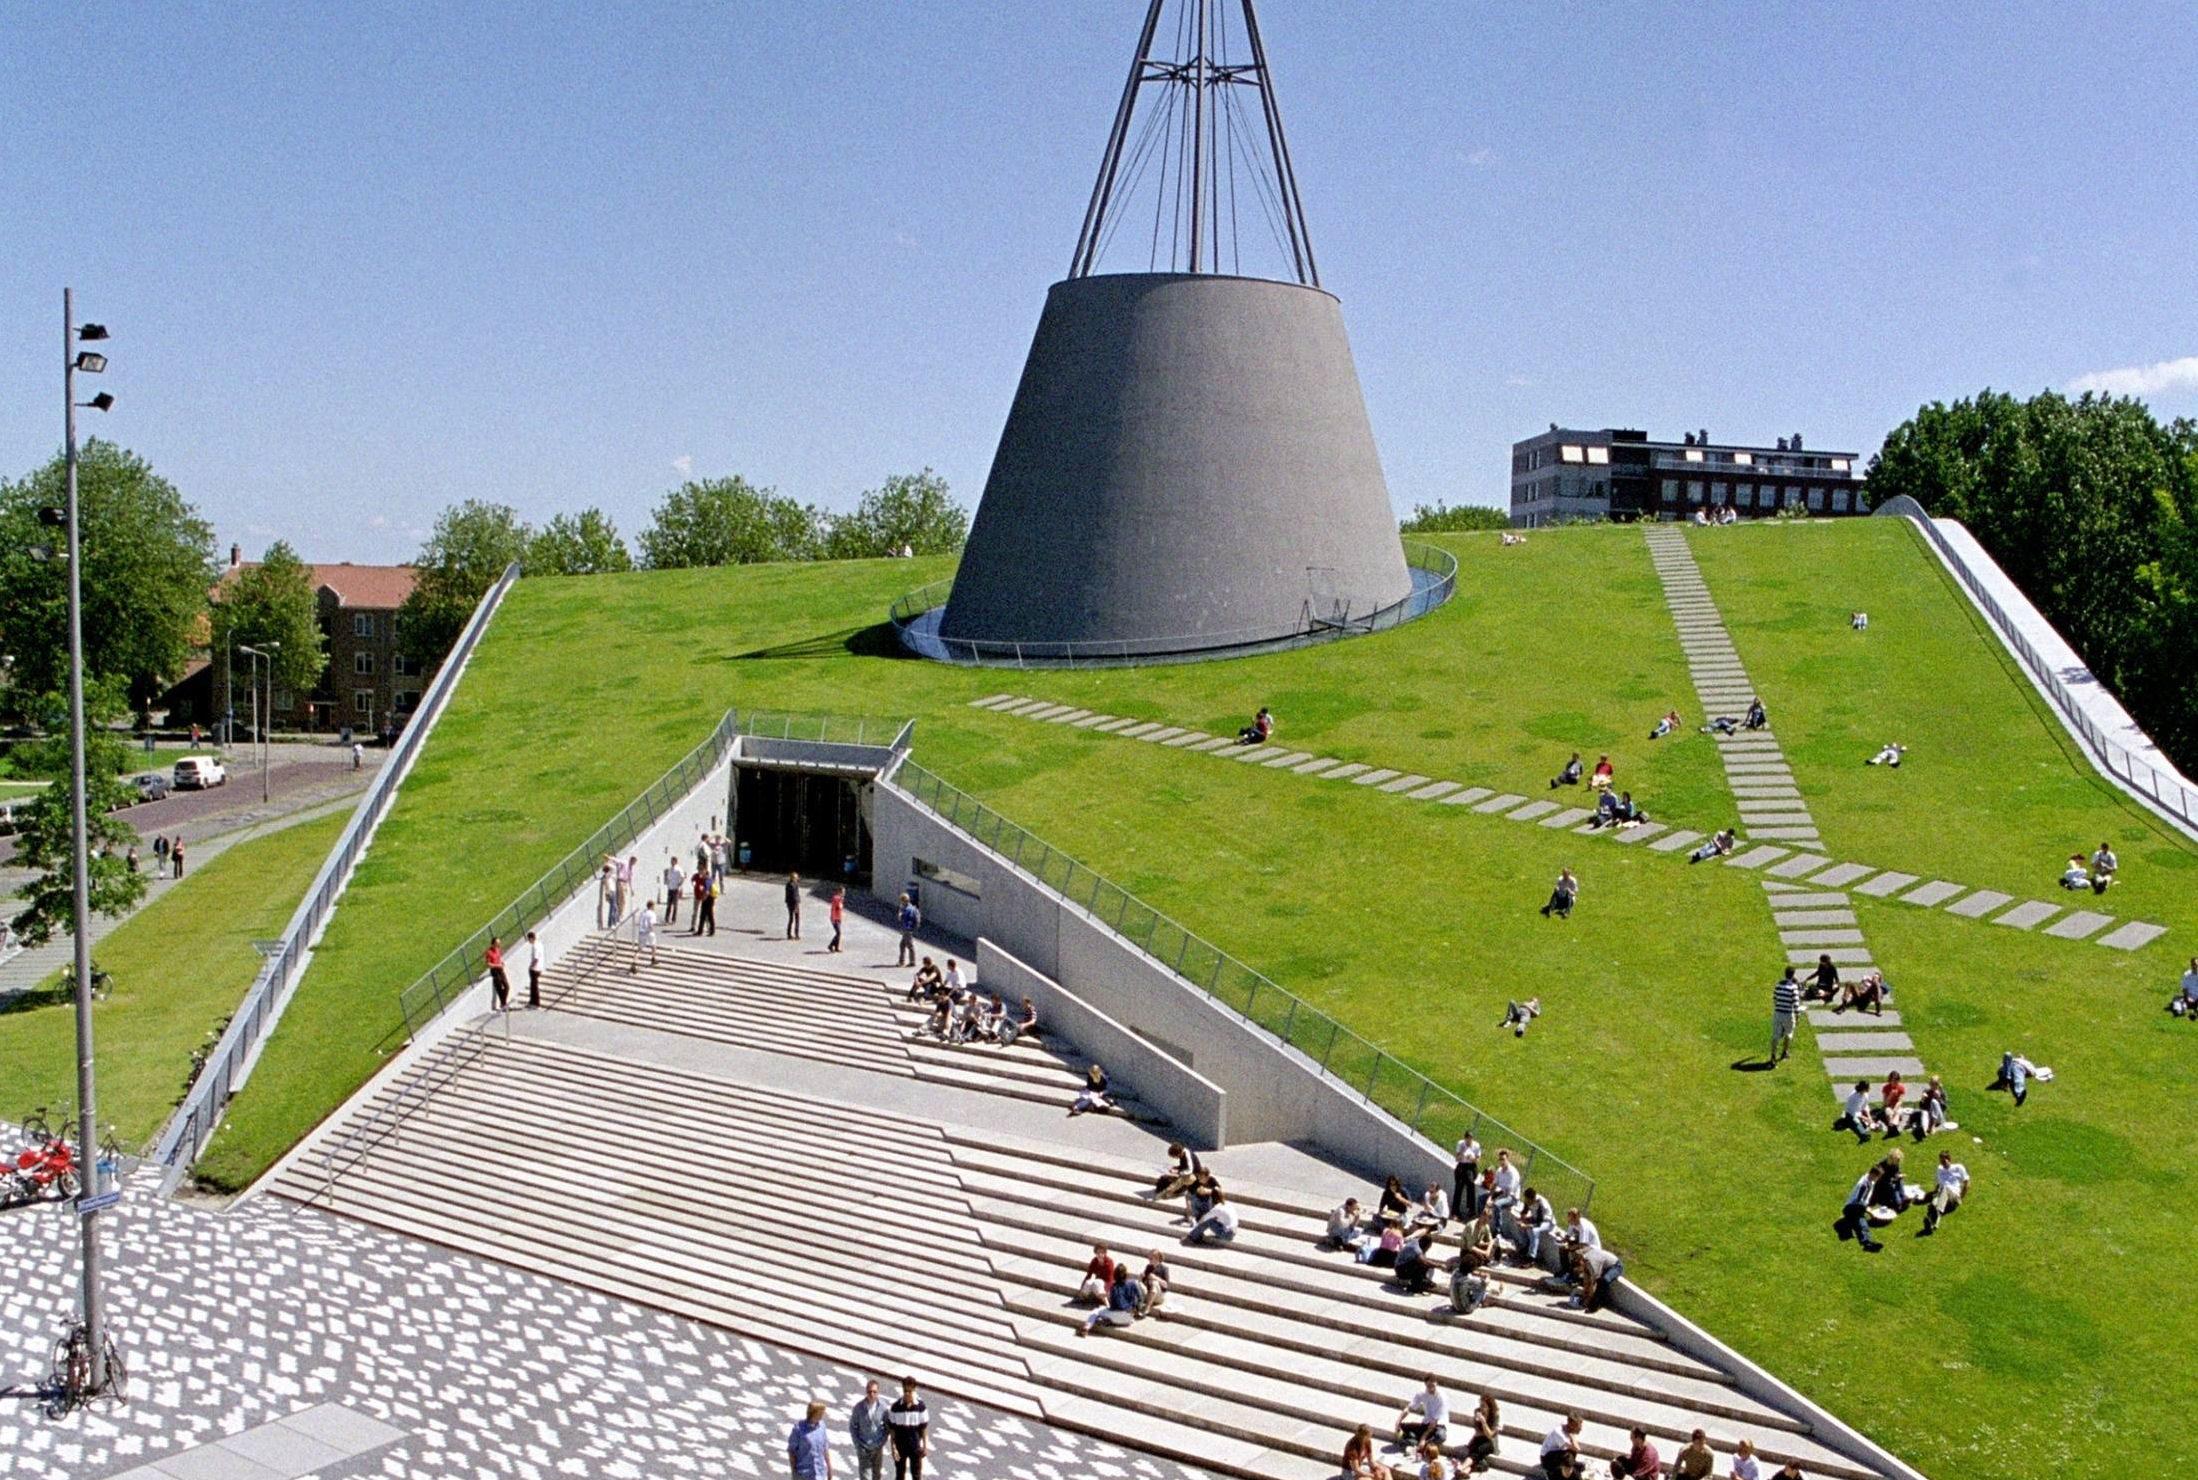
\includegraphics[width=\paperwidth,height=\paperheight]{images/background-titlepage.jpg}}%
	\setbeamertemplate{footline}{\usebeamertemplate*{minimal footline}}
	\frame{\titlepage}
}

\beamertemplatenavigationsymbolsempty
%\setbeamertemplate{navigation symbols}{}

\setbeamertemplate{caption}{\raggedright\insertcaption\par}

%{\setbeamertemplate{footline}{\usebeamertemplate*{minimal footline}}
%\begin{frame}\frametitle{\titleTOC}
%	\tableofcontents
%\end{frame}
%}

%\section{First Section}
%\subsection{Section 1 - Subsection 1}


	%Transcript:
	%Energy consumption is an important problem.
	%If we want to reduce it, we must first understand what devices actually use energy.
	%Smart-meter can help in this aspect by telling the consumer which appliance uses how much energy
	%The meter does this by recognizing the unique energy signature of each appliance
	%For example: the washer dryer uses a large amount of power for a long time 
	%while in contrast, the refrigerator uses a small amount of power for a small amount of time but it does it with a certain period.
	%This is what is meant by the enrgy signatures of appliances.
	%Since the fridge and the washer have distinct signatures they can be recognized.

	\begin{frame}\frametitle{Energy Disaggregation}

		Energy consumption is a most pressing issue.

		\begin{itemize}

			\item To reduce it, understanding the usage of that energy is needed.

			\item Smart-meter can disaggregate the energy usage in a household.

			\item This is done by recognizing the unique signatures of appliances.

		\end{itemize}

		\begin{figure}[t]
			\centering
			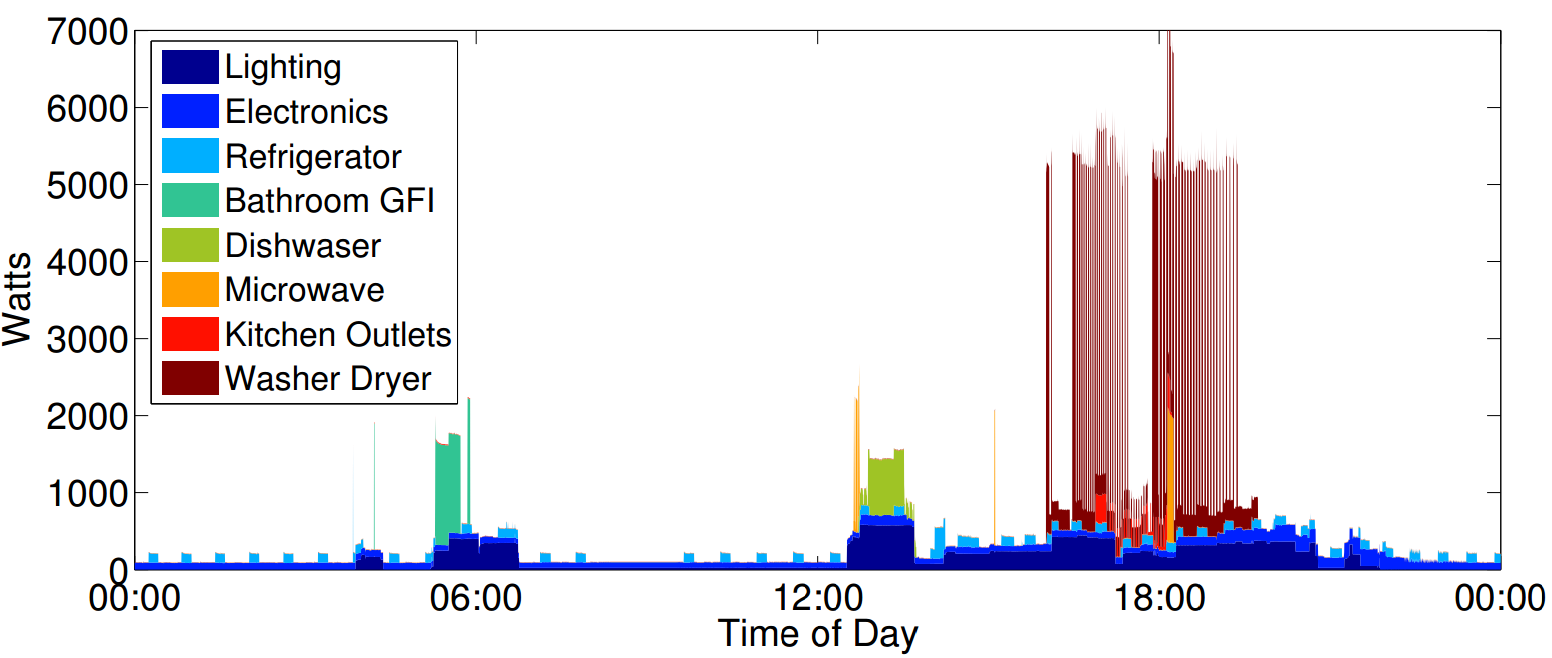
\includegraphics[width=0.7\textwidth]{../chapters/introduction-chapters/energy-consumption-house.png}
		\end{figure}


	\end{frame}



	%But individual lights can not be recognized, because lighting does not have unique signatures.
	%Instead many lights have the same signature making it impossible to recognize individual lights.
	%However it is still important to be able to recognize which individual lights are on because lightinh consumes about 20 % of the power in an avg household

	% So the key issue is that lights dont have a unique energy signature, so we must give them one.
	\begin{frame}\frametitle{Energy Consumption Lighting}

		Individual lights cannot be disaggregated (yet).

		\begin{itemize}

			\item The reason: Lighting does not have a unique signature. %Which HVAC for example does have.

			\item Instead there are many lights with the same signature.

			\item Still important to be able to disaggregate individual lights: Lighting consumes 19 \% of the power in an average household.

		\end{itemize}


	\end{frame}




	%VLC can help us with giving each light a unique signature.
	%VLC stands for visible light communication.
	%And it transmits data using lights by turning them on and off really fast so that no flickering effects can be seen.
	%Applications such as indoor localization use VLC to transmit positional data to for example a smartphone.
	%The phone can then determine its location inside a building where GPS can not.
	%Traditional VLC only cares about the data that is transmitted via light, it does not care about how that data translates into the current that each light draws.
	%But if we want to identify which light is on or off by the energy signature the current draw does become important.
	%Also the data or the IDs used to transmit becomes important, because the energy signatures of all lights are aggregated.
	%And we can only measure the aggregated signatures.


	\begin{frame}\frametitle{VLC Piggybacking}

		VLC is a communication method which uses visible light to transmit data.

		\begin{itemize}

			\item This data can be unique IDs for LED beacons used for indoor localization.

			\item This data will also propagate through the current draw.

			\item Can we construct these IDs in such a way that the aggregated current can be disaggregated by a smart-meter ?

		\end{itemize}


		\begin{figure}
			\centering
			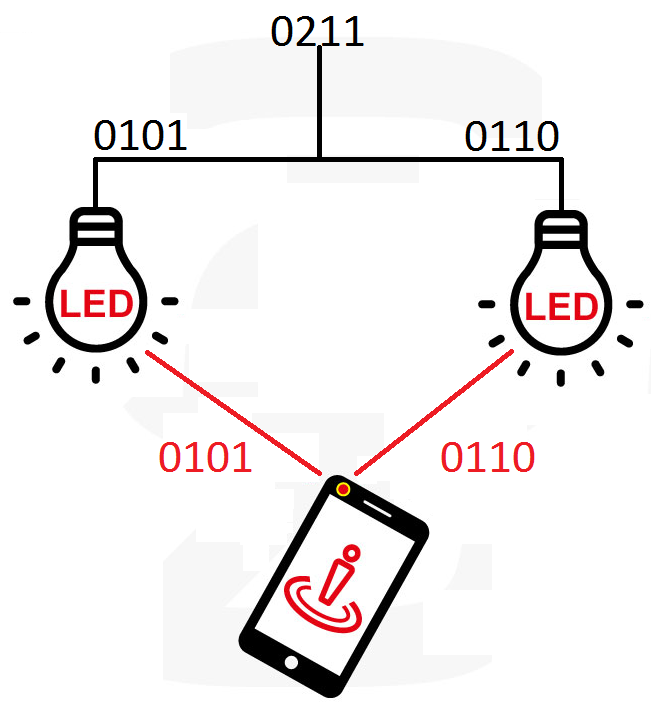
\includegraphics[width=0.3\textwidth]{vlc-indoor-positioning-edit.png}
		\end{figure}



	\end{frame}



	%And so weve come to the contributions of this work
	%First the IDs that can be used to indentify which lights are on and off are investigated.
	%Next, hardware is designed to let the IDs define the unique energy signature of each light.
	%Also a smart-meter is designed to measure the aggregated energy signatures of all the lights.
	%Finally the entire system is evaluated.

	\begin{frame}\frametitle{Contributions}


		%\begin{figure}
		%	\centering
		%	\resizebox {0.8\textwidth} {!} {
		%		\begin{tikzpicture}
		%			\node[block] (smart_meter) {Smart-meter};	
		%			\node[block, left = 1cm of smart_meter] (power) {Power};	
		%			\draw[line] (power.east) -- (smart_meter.west) node [midway, right] {};		
		%			% second mod.
		%			\node[block, right = 4cm of smart_meter] (second_modulator) {Modulator};
		%			\node[LED, right = 0.5cm of second_modulator] (second_led) {LED};
		%			\draw[line] (second_modulator.east) -- (second_led.west) node [midway, right] {};
		%			% first mod.
		%			\node[block, above = 1cm of second_modulator] (first_modulator) {Modulator};
		%			\node[LED, right = 0.5cm of first_modulator] (first_led) {LED};
		%			\draw[line] (first_modulator.east) -- (first_led.west) node [midway, right] {};
		%			% third mod.
		%			\node[block, below = 1cm of second_modulator] (third_modulator) {Modulator};
		%			\node[LED, right = 0.5cm of third_modulator] (third_led) {LED};
		%			\draw[line] (third_modulator.east) -- (third_led.west) node [midway, right] {};
		%			\node[dot, right = 2.5cm of smart_meter] (CP) {};
		%			\draw (smart_meter.east) -- (CP) node [pos=0.3, above] {0222};
		%			\draw (CP) |- (first_modulator.west) node  [pos=0.75, above] {0011};
		%			\draw (CP) |- (second_modulator.west) node [pos=0.75, above] {0110};
		%			\draw (CP) |- (third_modulator.west) node  [pos=0.75, below] {0101};
		%		\end{tikzpicture}
		%	}
		%\end{figure}

		\begin{figure}
			\centering
			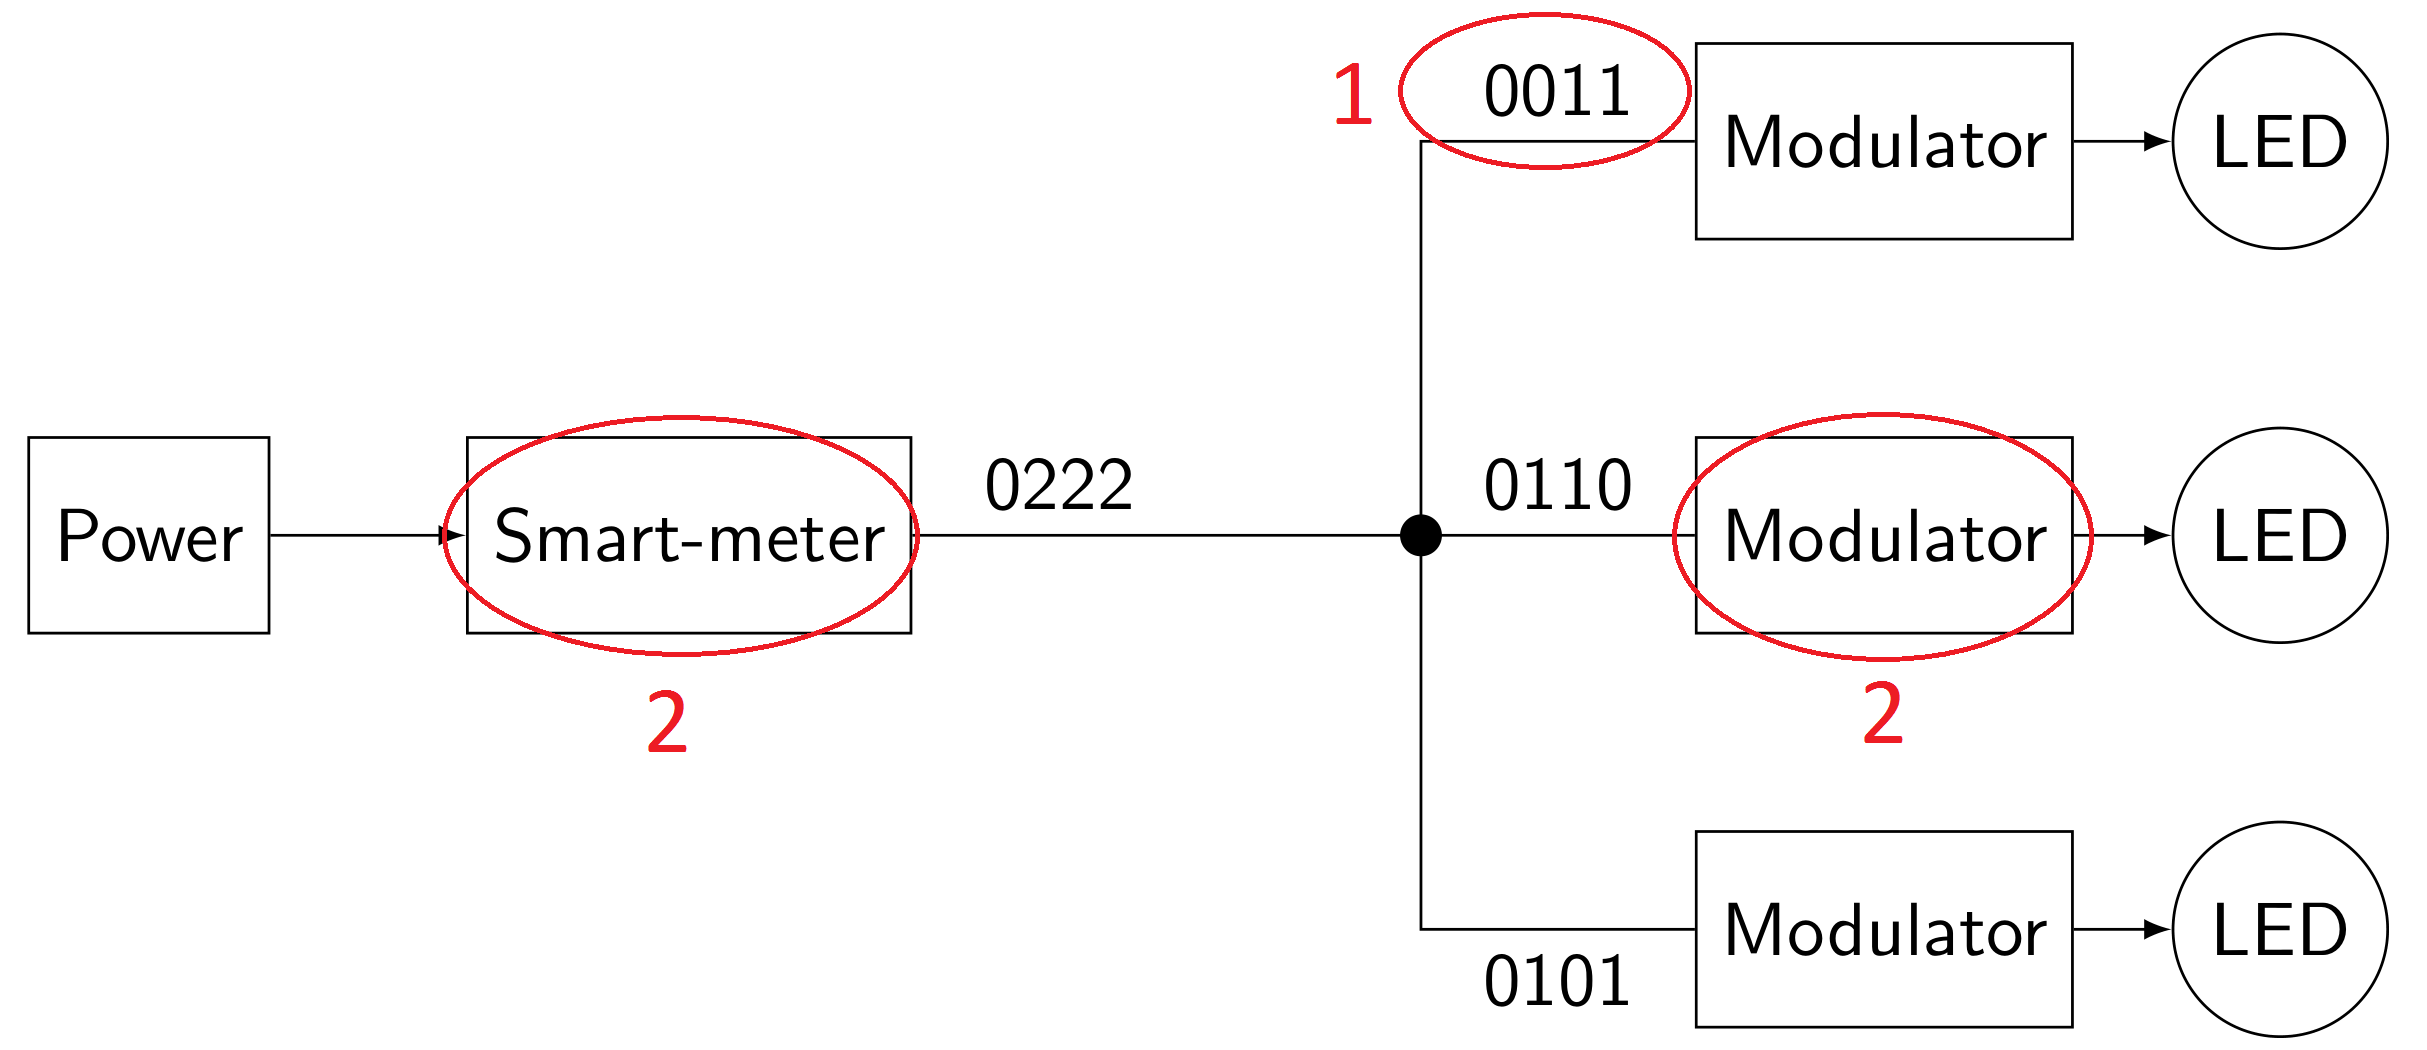
\includegraphics[width=\textwidth]{contributions-figure.png}
		\end{figure}

		\begin{enumerate}

				\item Investigation of codes that can be used.

				\item Design of hardware to modulate and sample the current.

				\item Evaluate the solutions.

		\end{enumerate}

		

		



		%\noindent
		%\begin{minipage}{.5\linewidth}
		%	
		%\end{minipage}%
		%\begin{minipage}{.5\linewidth}
		%	\begin{figure}
		%		%\centering
		%		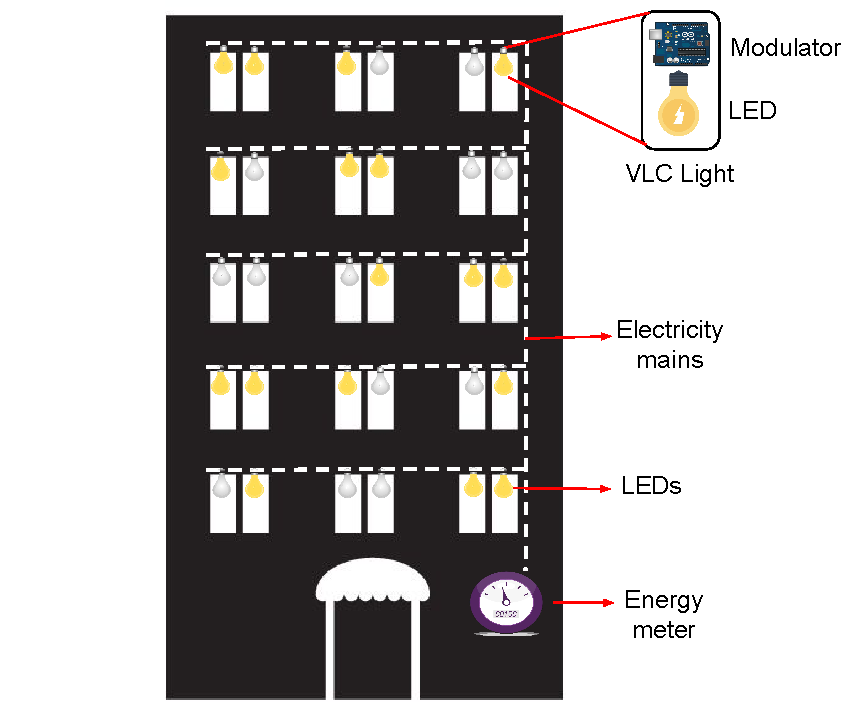
\includegraphics[width=1.05\textwidth]{design.pdf}
		%	\end{figure}
		%\end{minipage}

	\end{frame}



	%The problem were facing is that all the transmitters or LEDs in this case are transmitting on the same channal at the same time.
	%Also we can only measured the combined energy consumption.
	%But still we want to know which individual light is on or off.

	%There is a very similar problem with wireless communication.
	%Where multiple cellphones transmit to the same base station at the same time.
	%The base station also only receives the combined data.
	%But it still needs to figure out the data that each phone sent.
	%To solve that problem they use CDMA codes.

	%So to solve our problem problem we can also look at the cdma codes.
	%But to see which codes is the best we can first set some requirements.




	\begin{frame}\frametitle{Code Investigation}

		\begin{itemize}
			\item Problem:
			\begin{itemize}

				\item Multiple transmitters (LEDs) on the same channel at the same time.

				\item Only the aggregated energy can be measured.
			\end{itemize}

			\item Very similar to:

			\begin{itemize}

				\item Multiple cell phones transmitting to the same base station.

				\item Base station receives the combined signals.

			\end{itemize}
		\end{itemize}

	\end{frame}



	%The requirements that we need are the following:
	%The method to produce the codes must be scalable, meaning if we have a code length L, 2^L combinations of codes exist
	%But only a small subset of those can be used due to their resilience to the other LEDs which are also transmitting.

	%The codes that will be used must also have good balance properties.
	%For telecommuncications the number of consecutive zeros is not important, but for VLC it is important.
	%If there are too many consecutive zeros in a row, flickering effects may be observerd.

	%Lights can be turned on at the same time for example if they are in the same room.
	%But lights in different rooms can be turned on at different times.
	%In both cases the codes should perform well.

	%Since each code can be transmitted concurrently with another code, they should have low cross-correlation or high resilince to each other.


	\begin{frame}\frametitle{Requirements for Codes}
		
		\begin{itemize}

			\item Scalability

			\item Balance

			\item Synchronous and Asynchronous

			\item Resilience
			
		\end{itemize}
		
	\end{frame}






	
	
	%This is what I mean with correlation:

	%Correlation measures the similarity between the aggregated energy consumption and the ID of an LED.

	%For instance if we have three LEDs, A B and C, and they are all transmitting that they are on, we get an aggregated signal S which consitst
	% out of the IDs from LED a b and c.
	%To find out if LED A is on, we have to correlate the signal S with the ID A.
	%This produces some number which tells us if led A is on or off.
	%But this consists out of the correlation between A and A, A and B and A and C.
	% R_AA is called the auto-correlation, which should be a high number to identify of the LED is on or off.
	% The other two numbers are the cross-correlation, because the measure similarity between two different IDs.
	% These two terms cause interfence and limit the accuracy of the system, so the cross-correlation must be as low as possible.

	% Because we are dealing with a large amount of lights, the interference can be so high that we can not make sense of the aggregated signal anymore.
	% To prevent we will two solutions have been thought of which well come back to later.

	%Now that we have stated all the requirements for the codes we can look at the cdma codes themselves to see if they fulfill all of our requirements

	\begin{frame}\frametitle{Correlation}
		
		Measuring the similarity between a code and a received signal:

		\begin{equation*}
			R(\tau)_{xs} = \displaystyle\sum_{i = 0} ^ {L - 1} x(i) \times s(i + \tau) {\text{  with $\tau = 0, 1, 2, \dotsc, L$}}
		\end{equation*}

		

		%\noindent
		\vspace{10mm}
		\begin{minipage}{.5\linewidth}
			\begin{figure}
				\centering
				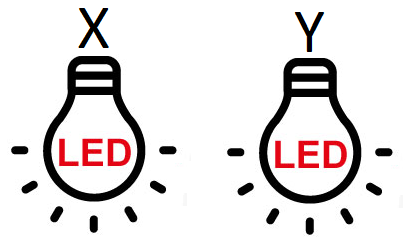
\includegraphics[width=0.8\textwidth]{correlation-leds.png}
			\end{figure}
		\end{minipage}%
		\begin{minipage}{.5\linewidth}
			\begin{itemize}
				\item $S = A + B + C$

				\item $R_{AS} = R_{AA} + R_{AB} + R_{AC}$

			\end{itemize}
		\end{minipage}

		%\begin{itemize}
%
%		%	\item Auto-correlation: When the ID is present in the signal, it should yield a high value.
%
%		%	\item Cross-correlation: When the ID is NOT present in the signal, it should yield a low value.
%
		%\end{itemize}


	\end{frame}



	
	%First we take a look at orthogonal codes.
	%These codes are used when transmitting from the base station to the cell phones.

	% These codes are created using a hadamard matrix.
	% This is a recursive square matrix, where each row represents a code and the number of columns is the length of the code.
	% Since this is a square matrix, the number of usable codes is propertional to the length of a code, so these codes are scalable.

	% But because the codes are generated recursively the number of consective zeros becomes larger and larger as the length of the code increases.
	% So they dont have the balance property 

	% these codes are called orthogonal codes because they have the property that each code is orthogonal to each other meaning the cross-correlation is zero.
	% However this is only the case when the codes are sent synchrounsly

	% But we require that the codes also work in asynchronous envoiroments
	% So lets take a look at a code that does just that:




	\begin{frame}\frametitle{Orthogonal Codes}
		\begin{itemize}

			\item Creation via Hadamard matrix: 
			\begin{equation*}
				H_{2n} = 
				\begin{bmatrix} 
					H_n & H_n \\ 
					H_n & \overline{H_n} 
				\end{bmatrix}
			\end{equation*}


			\noindent
			\begin{minipage}{.5\linewidth}
				\begin{equation*}
					H_{1} = 
					\begin{bmatrix} 
						1
					\end{bmatrix}
				\end{equation*}
			\end{minipage}%
			\begin{minipage}{.5\linewidth}
				\begin{equation*}
					H_{2} = 
					\begin{bmatrix} 
						1 & 1 \\ 
						1 & 0
					\end{bmatrix}
				\end{equation*}
			\end{minipage}

	
			\item Properties:
				\begin{itemize}


				\item Scalable: \cmark

				\item Balance: \xmark

				\item Correlation: \cmark  \  (Only synchronous)

				

			\end{itemize}


		\end{itemize}
		

	\end{frame}



	% pseudo random noise codes are generated by a linear feedback shift register.
	% By applying a suitable polynomial C to this register we get a code as output.

	% The number of codes that can be constructed this way is function of the primes of the length of the code.
	% So the relation is not linear, so these codes are not scalable.

	%But these codes do have the property that no matter the length there wont be a large amount of consecutive zeros
	% So it does have the balance property.

	% As apposoed to the orthogonal codes, these codes do allow for asynchronous transmission due to their good auto-correlation properties.
	% However they dont have good cross-correlation properties and this will limit the accuracy of the system.

	% TO solve the scalability and correlation issue, Gold codes were introduced:




	\begin{frame}\frametitle{PN Codes}
		\begin{itemize}
			\item Creation of a PN code via LFSR:
		
				\begin{figure}[t]
					\centering
					\resizebox {0.8\textwidth} {!} {
						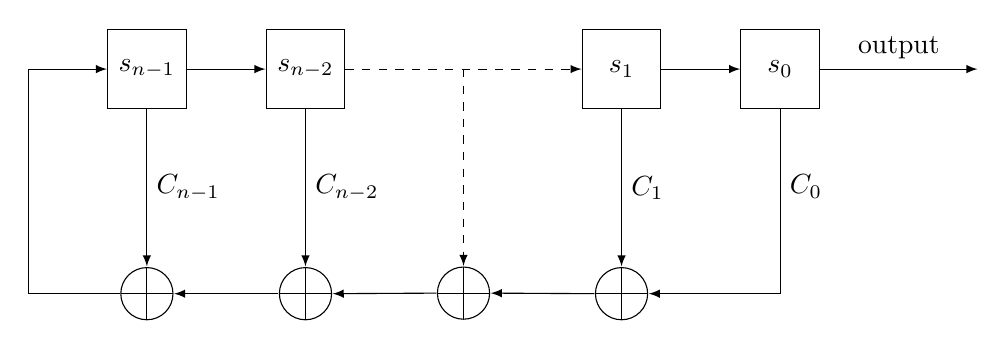
\begin{tikzpicture}


							\node[block                  ] (last_register) {$s_{n-1}$};
							\node[block, right = 1cm of last_register] (second_last_register) {$s_{n-2}$};
							\draw[line] (last_register.east) -- (second_last_register.west) ;

							\node[block, right = 3cm of second_last_register] (second_register) {$s_{1}$};
							\node[block, right = 1cm of second_register] (mid_register) {$s_{0}$};
							\draw[line] (second_register.east) -- (mid_register.west) ;

							\draw[dashed, line] (second_last_register.east) -- (second_register.west) ;

							\node[coordinate, right = 2cm of mid_register] (output_point) {};
							\draw[line] (mid_register.east) -- (output_point.west) node [midway, above] {output};

							\node[XOR, scale=2, below = 2cm of second_register] (first_xor) {};
							\draw[line] (second_register.south) -- (first_xor.north) node [midway, right] {$C_1$};
							\draw[line] (mid_register.south) |- (first_xor.east) node [pos=0.21, right] {$C_0$};

							\node[coordinate, right = 1.5cm of second_last_register] (h) {};
							\node[XOR, scale=2, below = 2.5cm of h] (mid_xor) {};
							\draw[line] (first_xor.west) -- (mid_xor.east) ;
							\draw[dashed, line] (h.south) -- (mid_xor.north) ;

							\node[XOR, scale=2, below = 2cm of second_last_register] (second_last_xor) {};
							\node[XOR, scale=2, below = 2cm of last_register] (last_xor) {};

							\draw[line] (second_last_register.south) -- (second_last_xor.north) node [midway, right] {$C_{n-2}$};
							\draw[line] (mid_xor.west) -- (second_last_xor.east) ;
							
							\draw[line] (second_last_xor.west) -- (last_xor.east) ;
							\draw[line] (last_register.south) -- (last_xor.north) node [midway, right] {$C_{n-1}$};

							\node[coordinate, left = 1cm of last_register] (return_point) {};
							
							\draw[line] (last_xor.west) -| (return_point) -- (last_register.west) ;

						\end{tikzpicture}
					}
				\end{figure}

			\item Properties:

			\begin{itemize}

				\item Scalable: \xmark

				\item Balance: \cmark

				\item Auto-correlation: \cmark

				\item Cross-correlation: \xmark



				%\item Auto-correlation is high, in synchronous and asynchronous scenarios.

				%\item Cross-correlation: Exhaustive analysis is required.

				%\item Number of codes $C = \frac{1}{n} \prod \{ P_{i} ^ {(\alpha_i - 1)} \times (P_i - 1) \}$ $\rightarrow$ $C \not\propto L$, does not scale well.
			\end{itemize}

		\end{itemize}
		

	\end{frame}



	% Gold codes are created using two LFSRs, but is too complicated to show in this presentation.
	% But due to this creation method the scalabilty issue of the PN codes is solved.

	%Due to the similar construction method as PN codes, they also retain the balance property.

	% Finally, these codes have good auto and cross correlation properties which will allow multiple LEDs to transmit at the same time without effecting the accuracy of the system. Also the cross correlation is math. bounded.


	% Since the gold codes fulfill of our requirements, we will use these codes in our system.

	\begin{frame}\frametitle{Gold Codes}

		\begin{itemize}
			\item Creation of a Gold code via two LFSRs.

			\item Properties:
			\begin{itemize}

				\item Scalable: \cmark

				\item Balance: \cmark

				\item Auto-correlation: \cmark

				\item Cross-correlation: \cmark


			\end{itemize}


		\end{itemize}
		

	\end{frame}










	%\begin{frame}\frametitle{Comparison of Codes}
	%	\begin{table}
	%		\centering
	%		\resizebox {\textwidth} {!} {
	%			\begin{tabular}{ | l | l | l | l | }
	%				\hline
	%																& Orthogonal 	& PN 		& Gold 		\\ \hline
	%				Synchronous	Transmission						& \cmark		& \cmark	& \cmark	\\ \hline
	%				A-synchronous Transmission						& \xmark		& \cmark	& \cmark	\\ \hline
	%				Math. bounded CC (synch.)						& \cmark		& \xmark	& \cmark	\\ \hline
	%				Math. bounded CC (asynch.)						& \xmark		& \xmark	& \cmark	\\ \hline
	%				Scalability ($C \propto L$)						& \cmark		& \xmark	& \cmark	\\ \hline		
	%			\end{tabular}
	%		}
	%	\end{table}
	%\end{frame}





	% Now that we have codes that fulfil our requirements we are face with the following issue.
	% These CDMA codes are used with wireless telecommunication with the cell phones for example
	% There they can use -1 and +1 symbols and on these symbols the correlation function is defined which i showed earlier.
	% On the left hand side you can see a simple code that is transmitted with +1 and -1 symbols for which we can use the normal correlation function.

	% However our leds cannot do +1 and -1 symbols.
	% They can only be turned on or off, so the can only use 0 and 1 symbols.
	% So a mapping must take place between these two sets of symbols.
	% That is done via this mapping formula.
	% Since we are now using different symbols the correlation function does not output the same results
	% instead we have a new function called r hat.
	% in order to get the same results as output we must transform r hat to the normal correlation function r.
	% the proof of this transformation can be found in the thesis.



	\begin{frame}\frametitle{Mapping Problem}

		\noindent
		\begin{minipage}{.5\linewidth}
			\begin{figure}
				\centering
				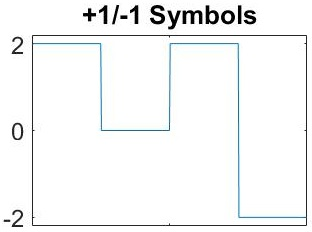
\includegraphics[width=0.8\textwidth]{mapping_radio_symbols.jpg}
			\end{figure}

			\begin{itemize}
				\item Normal correlation function: $R_{XY}$
			\end{itemize}
			
		\end{minipage}%
		\begin{minipage}{.5\linewidth}
			\begin{figure}
				\centering
				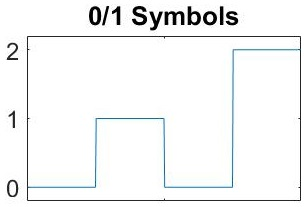
\includegraphics[width=0.8\textwidth]{mapping_binary_symbols.jpg}
			\end{figure}

			\begin{itemize}
				\item Mapping of symbols: $b = \frac{1 - r}{2}$
				\item New correlation function: $\hat{R}_{XY}$
				\item $R_{XY} = f(\hat{R}_{XY})$    %$R_{XY} = -m - 2 \times \hat{R}_{XY}$
			\end{itemize}


		\end{minipage}

	\end{frame}



	% now that we have found codes that fulfill our requirements
	% and that we are able to use them with LEDs trough mapping
	% we are left with one issue and that is interference from other transmitting LEDs.

	% This figure from earlier shows this interference.
	% Here we want to see if light A is on. 
	% but B and C are interfering with identifying if A is on or off.

	%becuse of the interfernce of other LEDs there must be a maximum amount of other leds transmitting at the same time while still maintaining an accurate system.

	% Because the Gold codes that we are using have a bounded cross-corraltion we calcalute the number of concurrent transmitting LEDs called $m$.
	% this calculation also provides a threshold for which we can decide if an LED is on or off
	% If correlation > T led is on and if lower the led is off.
	% now that we know what the maximum no. of transmitting LEDs is, we must make sure never to excedd m.

	%This can be done in via methods.
	%





	\begin{frame}\frametitle{Interference Solution}

		\begin{minipage}{.5\linewidth}
			\begin{figure}
				\centering
				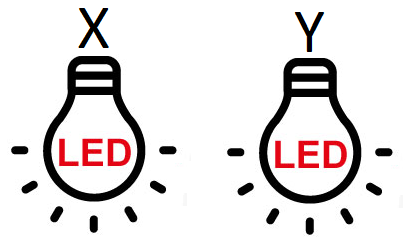
\includegraphics[width=0.8\textwidth]{correlation-leds.png}
			\end{figure}
		\end{minipage}%
		\begin{minipage}{.5\linewidth}
			\begin{itemize}
				\item $S = A + B + C$

				\item $R_{AS} = R_{AA} + R_{AB} + R_{AC}$

			\end{itemize}
		\end{minipage}
		\vspace{10mm}
		\begin{itemize}
			\item Determine max. no. of modulating LEDs $m = \frac{L}{2 \times \phi}$
			\item Threshold: $T = \frac{L}{2}$ %; $R > T$: LED on ; $R \le T$; LED off
			\item Make sure the no. of modulating LEDs $\le m$:
				\begin{itemize}
					\item Continuous Method
					\item Probabilistic Method
				\end{itemize}
		\end{itemize}


		%\begin{itemize}
		%	\item $R_{XY} \neq 0$ for Gold codes.
		%	\item $R_{XY}$ is bounded.
		%	\item Determine the max. no. of concurrent transmitters $m$ such that no interference occurs.
		%	\item Example:
		%		\begin{itemize}
		%			\item 1025 LEDs
		%			\item 1023 ID length
		%			\item $m = 7$ LEDs
		%		\end{itemize}
		%	\item Continuous Method: Allows to transmit with all LEDs continuously.
		%	\item Probabilistic Approach: Each LED will have a probability to transmit.
		%\end{itemize} 

		%Cross-correlation is not negligible, therefore there will be interference. The amount of interference must be limited to still get accurate results.

		%\begin{itemize}

		%	\item Continuous Method: Allows to transmit with all LEDs continuously.

		%	\item Probabilistic Approach: Each LED will have a probability to transmit.


		%\end{itemize}


	\end{frame}



	%The continous method makes sure that there will never be more than m modulating LEDs by only using a total of m LEDs in the system.
	%An appropiate code length is needed that supports these m LEDs.
	%Unfortunately L is proportial to m sqaured, so the time to indentify all LEDs in the system quickly blows up.

	%For example when using 7 LEDs we can identify all the leds withtin point o 5 seconds.
	% but for a thousand leds the time explodes to 14 minutes due to the long code that has to be used.

	\begin{frame}\frametitle{Continuous Method}

		%Cross-correlation is math. bounded with Gold codes, bounded meaning that the maximum number of concurrent transmitters $m$ can be calculated, such that no interference will take place.

		\begin{itemize}
			
			\item Maximum of $m$ LEDs in system.
			\item Appropriate code length: $L \propto m^2$.

			\item Examples with modulating frequency $f = 10$ kHz:
			\begin{itemize}


				\item $m = 7$ LEDs $\rightarrow L = 1023$ $\rightarrow t = 0.05$ s.
				\item $m = 1023$ LEDs $\rightarrow L = 2^{23} = 8388608$ $\rightarrow t = 14$ min.
			\end{itemize}
		\end{itemize}


	\end{frame}



	% in order to speed the system up, a probabilistic approach is used.
	% with this approach a trade off must be made betweeen time and accuracy.
	% The accuracy expressed in 1 - epsilon outputs a probability p which is assigned to each LED for which it will transmit.
	% p is chosen such that most of the time the number of transmitting leds will not exceed m.
	% when we have approx. the same number of LEDs as in the previous example where it took 14 mins, it will now take less than a minute with 99.9 accuracy or even faster 22 s for a slighty lower accuracy.
	



	\begin{frame}\frametitle{Probabilistic Approach}


		\begin{itemize}
			\item Accuracy ($1 - \epsilon$) outputs a probability $p$.
			\item $p$ is chosen such that no. of modulating LEDs $\le m$.
			\item Example:
				\begin{itemize}
					\item $1025$ LEDs $\rightarrow L = 1023$ $\rightarrow t = 53$ s for 99.9 \% accuracy or $t = 22$ s for 99 \% accuracy.
				\end{itemize}
		\end{itemize}

		%Trade-off must be made by the user between time and accuracy.
		%\begin{itemize}
		%	\item Accuracy ($1 - \epsilon$): determines the accuracy in identifying which LEDs are on and off. Outputs a probability $p$ for which the LEDs will modulate.
		%	\item Each point in time the no. of modulating LEDs $\le m$.
		%	\item Time it will take to successfully identify all LEDs: $t = \frac{L}{f} \times \frac{1}{p}$
		%	\begin{itemize}
		%		\item Example: $1025$ LEDs $\rightarrow L = 1023$ $\rightarrow t = 53$ s for 99.9 \% accuracy or $t = 22$ s for 99 \% accuracy.
		%	\end{itemize}
		%\end{itemize}
		
	\end{frame}




	% Now we are done with invesitgating the codes.
	% We now have codes that fulfill our requirements, we can use them with LEDs trough mapping and we can indentify a large amount of leds in a timely manner.
	% Or at least we can do this in theory.

	% now we need to investigate if it will also work in practice
	% To do this we will need two pieces of hardware: the modulator and the smart-meter.

	% first we will go over the modulators requirements


	\begin{frame}\frametitle{Hardware Components}


		\begin{figure}
			\centering
			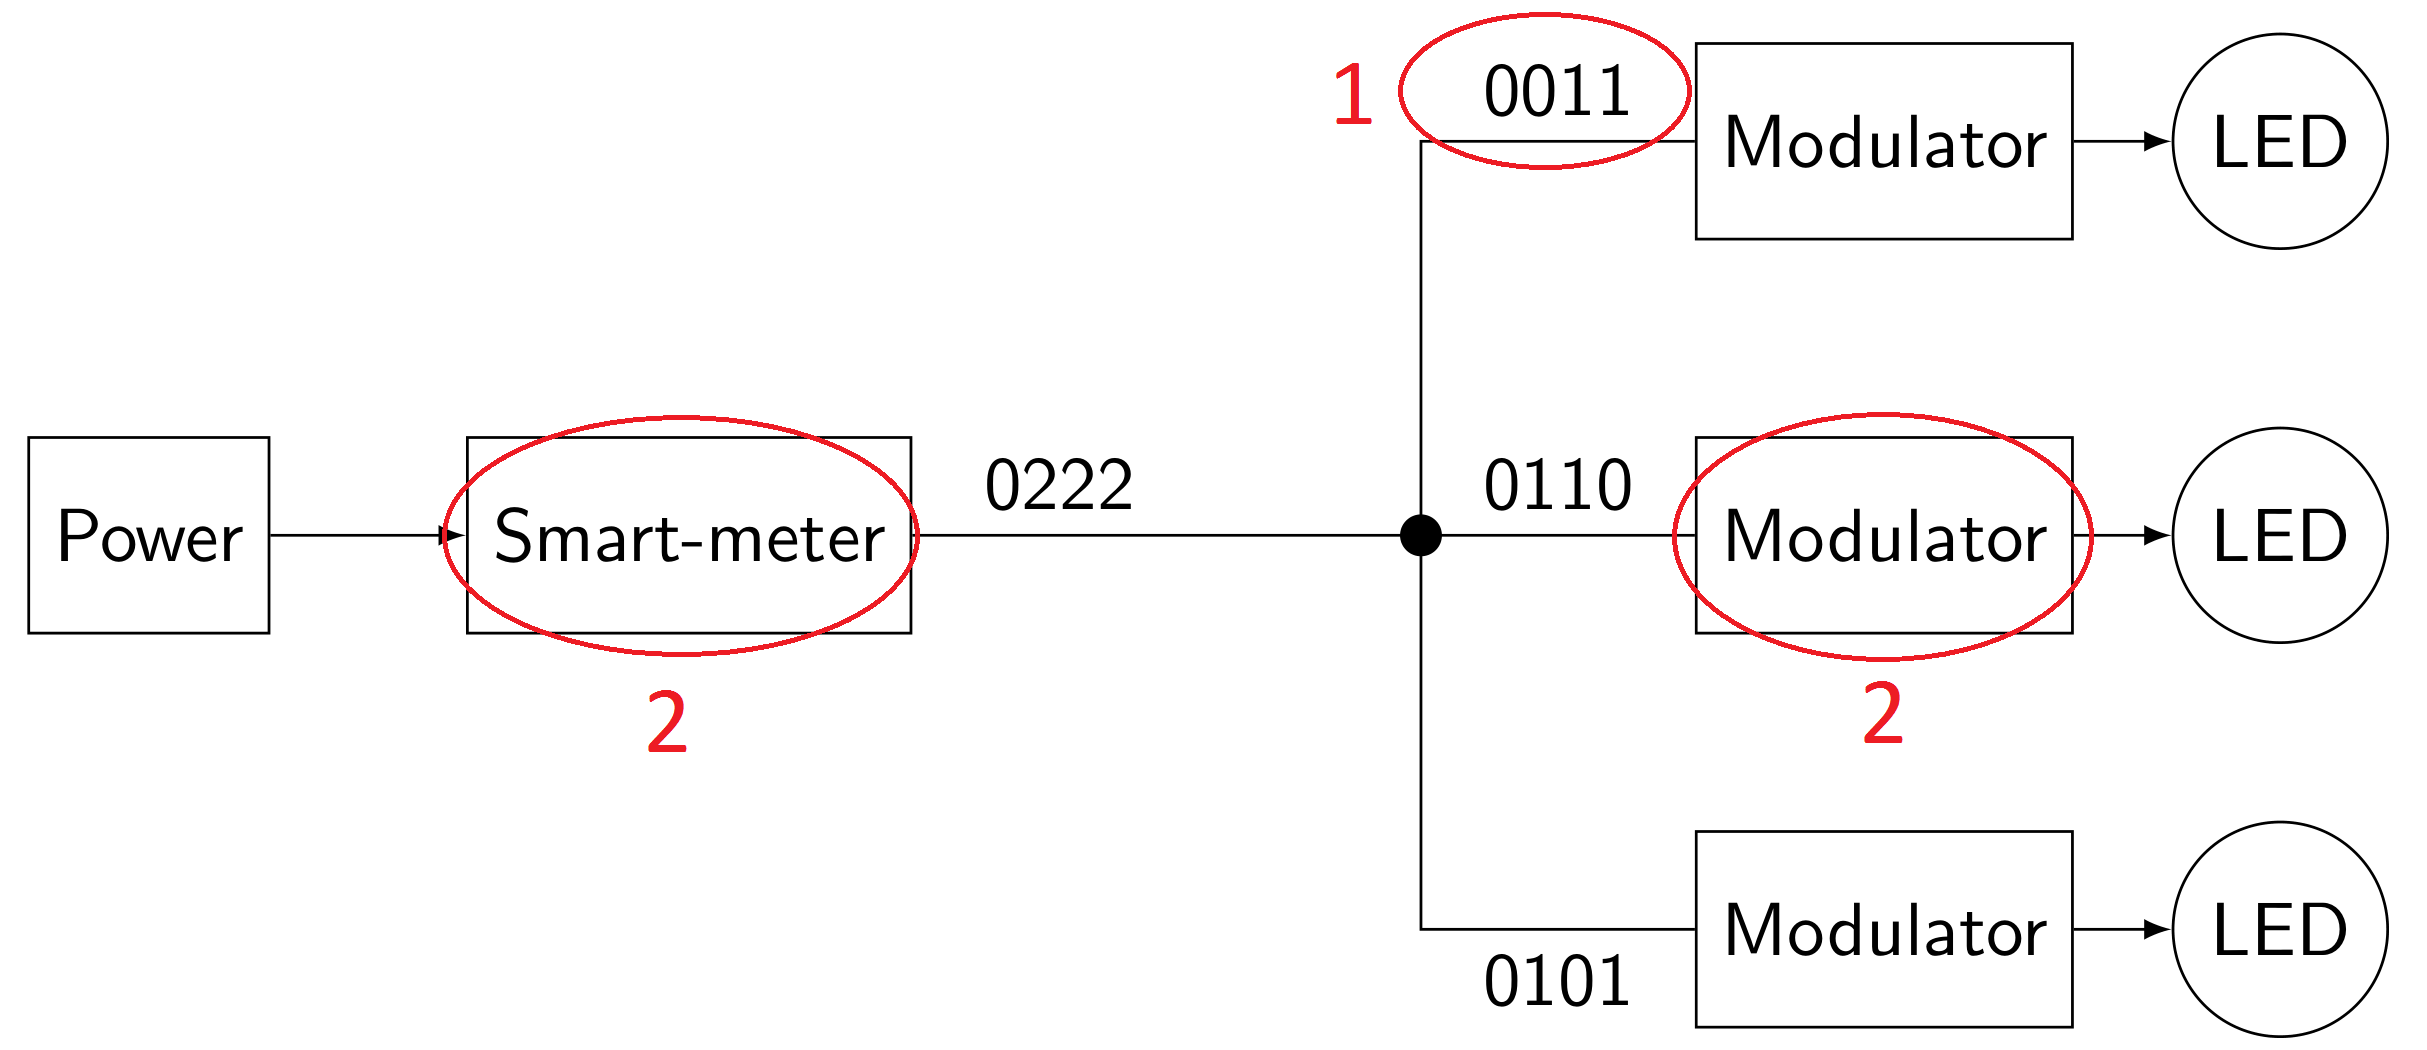
\includegraphics[width=\textwidth]{contributions-figure.png}
		\end{figure}
		\begin{enumerate}
				\item Codes
				\item Hardware
		\end{enumerate}
	\end{frame}



	% the modulator must tanslate the ones and zeros of the ID into the energy signature.
	% ideally we want when encoding a 0 no current draw.
	% and when encodiong a 1 we want som constant current draw for the duration of this symbol.

	% OF cource hardware already exists that can modulate an LED to transmit data with VLC.
	% And this works fine when only using VLC, but we also care about the translation from that data into the current draw.

	% So we will look at the energy signature of existing hardware.

	\begin{frame}\frametitle{Modulator Requirements}
		Modulator must translate ones and zeros of ID into current draw.
		\begin{itemize}
			\item $0 \rightarrow$ no current draw.
			\item $1 \rightarrow$ some constant current draw.
		\end{itemize}
	\end{frame}




	% Here the energy signature is shown of an Switching power supply when encoding a zero and a one.
	% these power supplies are used due to their high effiency.
	% but they do not meet our requirements for translating the ID into current.

	\begin{frame}\frametitle{Existing Modulator Hardware}

		\begin{figure}
			\resizebox {0.8\textwidth} {!} {
			  \centering
			  \begin{minipage}[b]{0.48\textwidth}
			    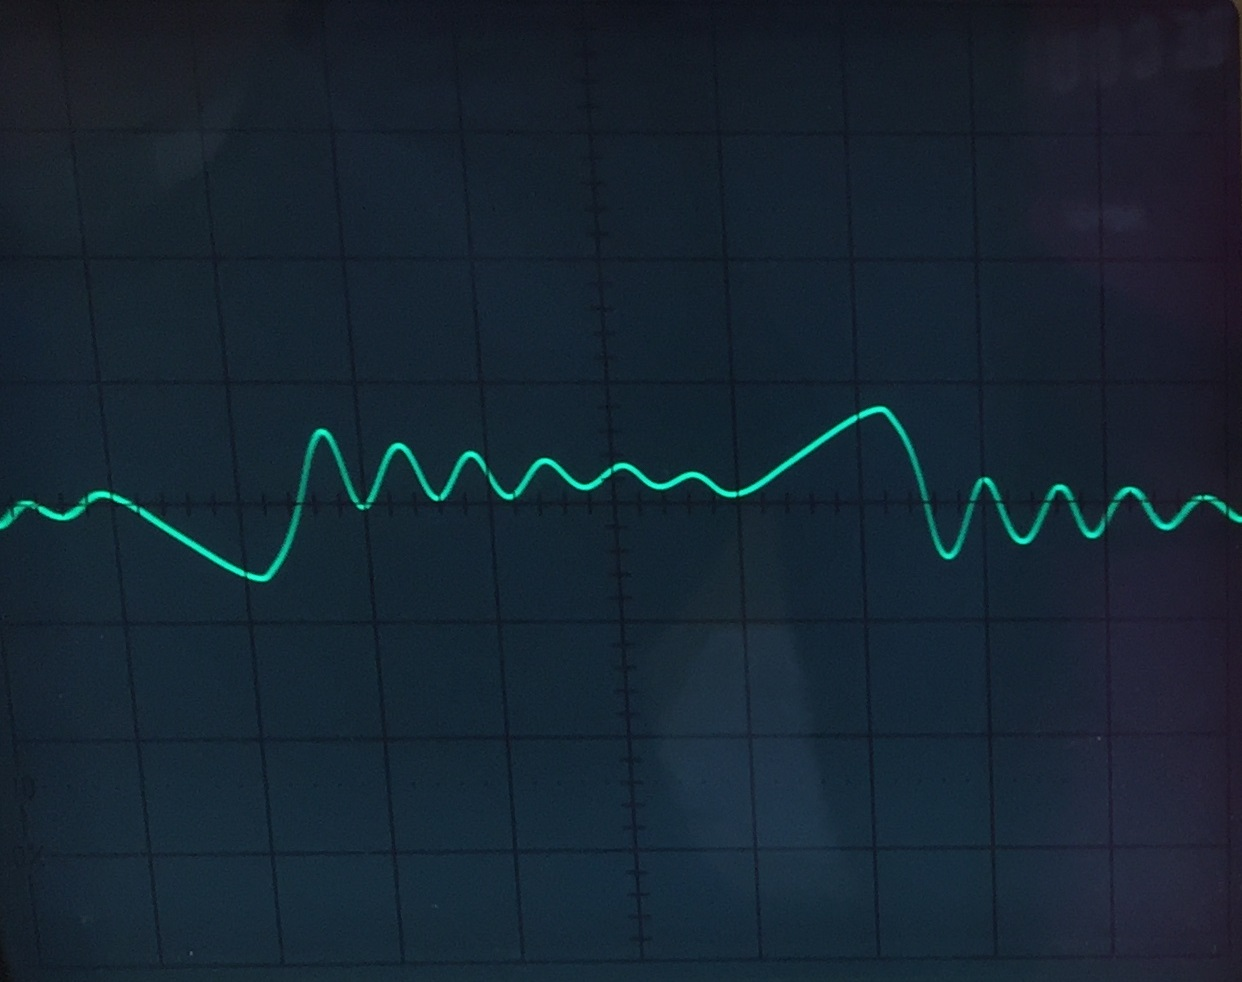
\includegraphics[width=\textwidth]{../chapters/hardware-chapters/AC/ac-modulator/smps-led/smps-current-primary-no-load-cropped.jpg}
			    \caption{Switching Mode Power Supply modulating a `0'}
			  \end{minipage}
			  \hfill
			  \begin{minipage}[b]{0.48\textwidth}
			    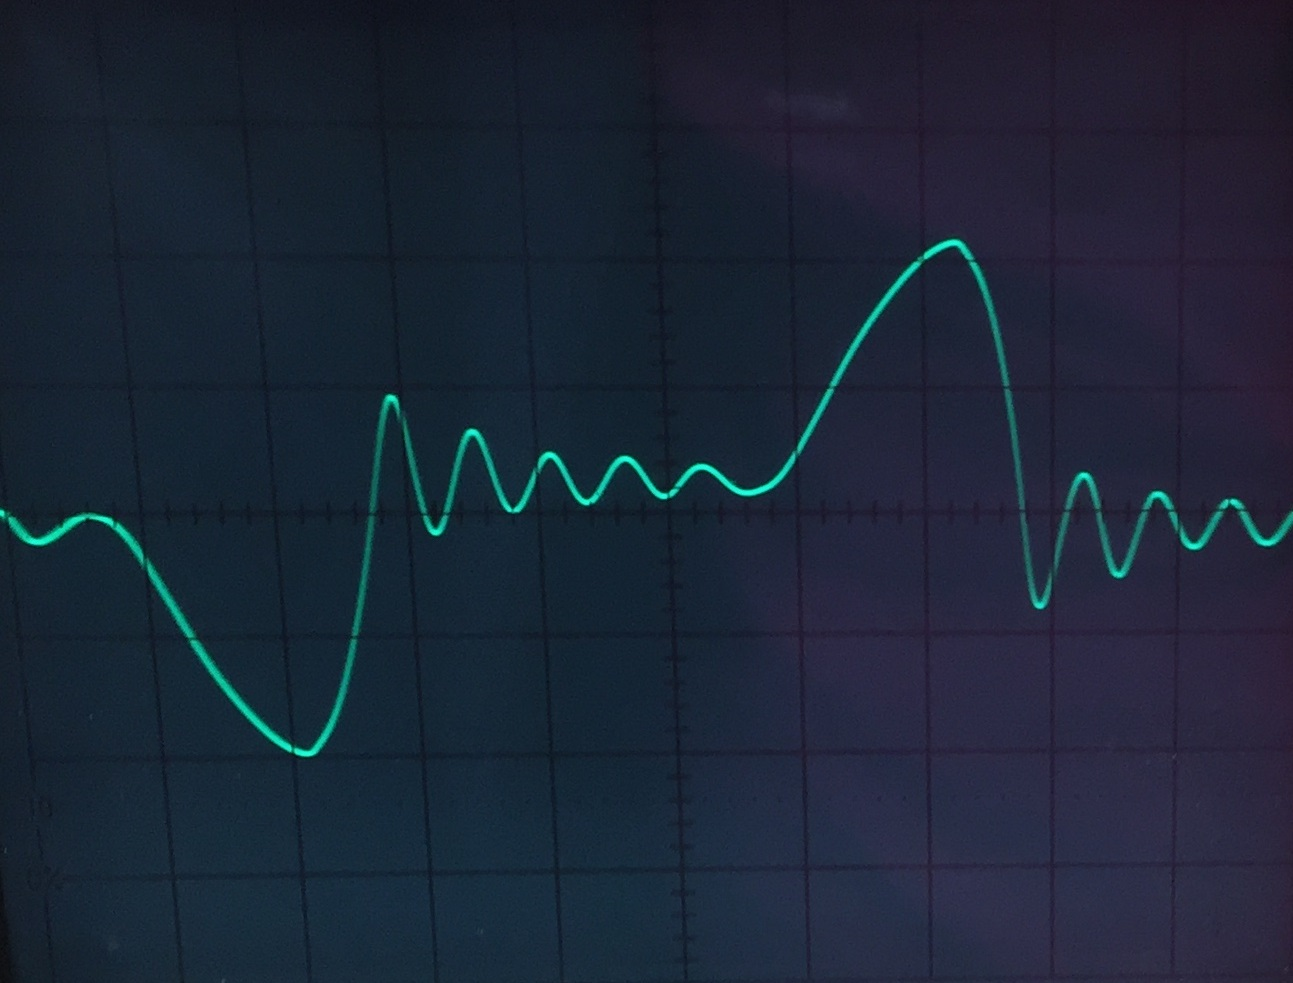
\includegraphics[width=\textwidth]{../chapters/hardware-chapters/AC/ac-modulator/smps-led/smps-current-primary-with-load-cropped.jpg}
			    \caption{Switching Mode Power Supply modulating a `1'}
			  \end{minipage}
		  }
		\end{figure}

		Very hard to distinguish and will not yield nice aggregated results when multiple of these SMPS will be used.
		
	\end{frame}


	% So it was decided to build our own LED modulator.
	% an overview of which can be seen here
	% The modulator consists of two major parts: The triggering circuit, the current source.
	% The purpose of each part will be explained shortly.
	% The way it workd is as follows: the triggering circuit tells the micro controller when to start and stop transmitting the ID.
	% and the micro controller encodes the ID by telling the current to turn on and off accordingly.



	\begin{frame}\frametitle{Custom Modulator}
		\begin{figure}
			\centering
			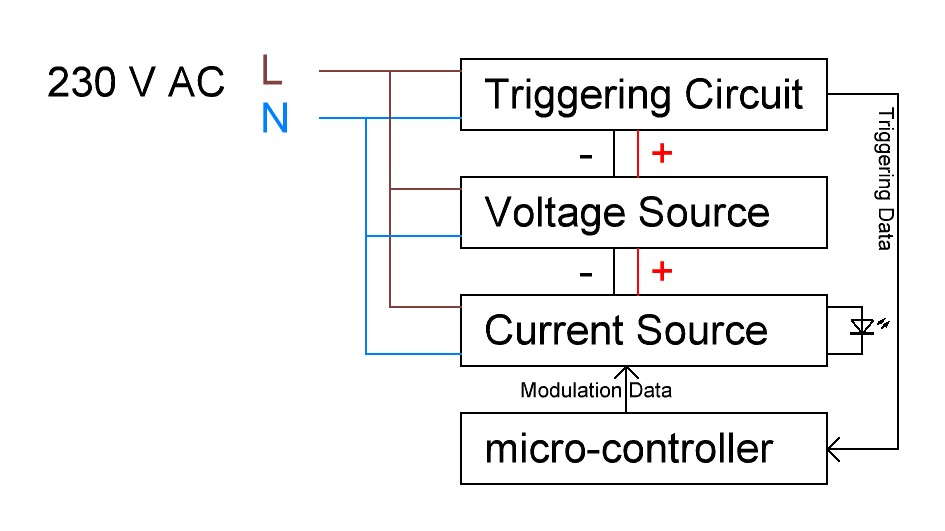
\includegraphics[width=0.8\textwidth]{../chapters/hardware-chapters/AC/ac-modulator/custom-hardware/ac-modulator-architectural.JPG}
		\end{figure}
	\end{frame}





	%the triggering circuit is needed because we are dealing with alternating voltage.
	% The AC voltage can be seen in the figure by looking at the sine wave.
	% It can be seen that the voltage is not a constant.

	% another thing we need to consider is that LEDs require a certain amount of voltage before they draw current.
	% This voltage can also be seen in the figure by the blue and red lines.
	% whenever the sine wave is below this voltage no modulation must take place because the LED will not draw current at that time and thereby losing information

	%but whenever the voltage is higher than the preset voltage, modulation can take place.
	% whenever it is above the blue line for example, we can modulate the LED.

	% this is exactly what the triggering circuit does.
	% it compares the incoming AC voltage and the preset voltage
	% and lets the micro contoller know when to start and stop modulating as seen from the orange line.


	\begin{frame}\frametitle{Detecting When to Modulate}
		\begin{itemize}
			\item AC Voltage is zero crossing.
			\item LEDs require some voltage before the current starts flowing.
		\end{itemize}
		
		\begin{figure}
			\centering
			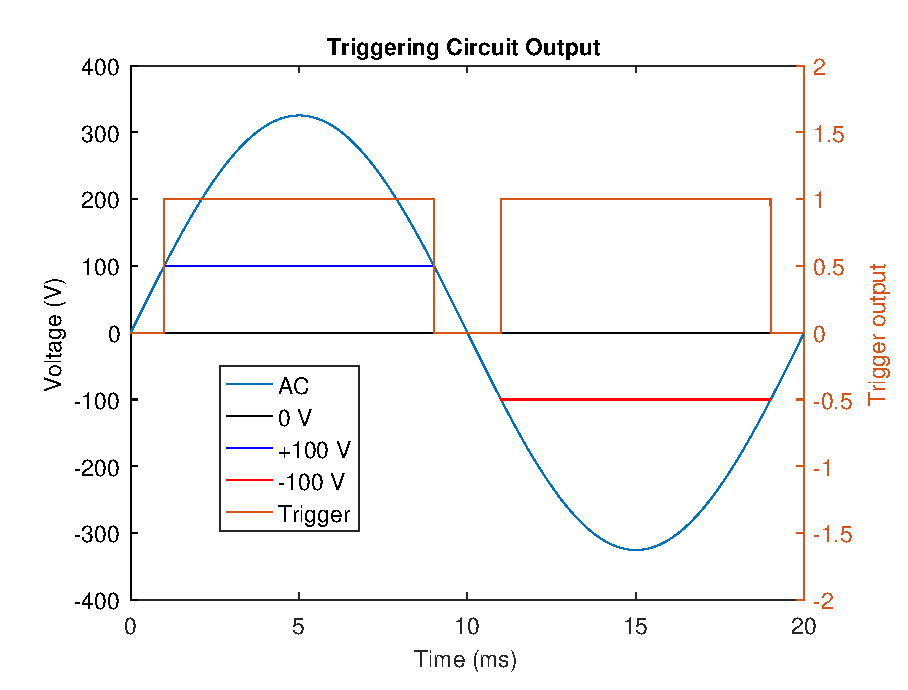
\includegraphics[width=0.7\textwidth]{ac-wave-triggering.eps}
		\end{figure}
		
	\end{frame}


	% the other major part is the current source.
	% whenever the micro controller is modulating the ID we wanted to have zero current when encodong a zero and some constant when encoding a one.
	% this is exactly what the current source does.
	% in the figure consecutive zeros and ones are encoded and for each symbol it is constant for the duration of that symbol.


	\begin{frame}\frametitle{Constant Current Draw}
		\begin{itemize}
			\item AC Voltage is not constant.
			\item For disaggregation a constant current is desired.
		\end{itemize}
		\begin{figure}
			\centering
			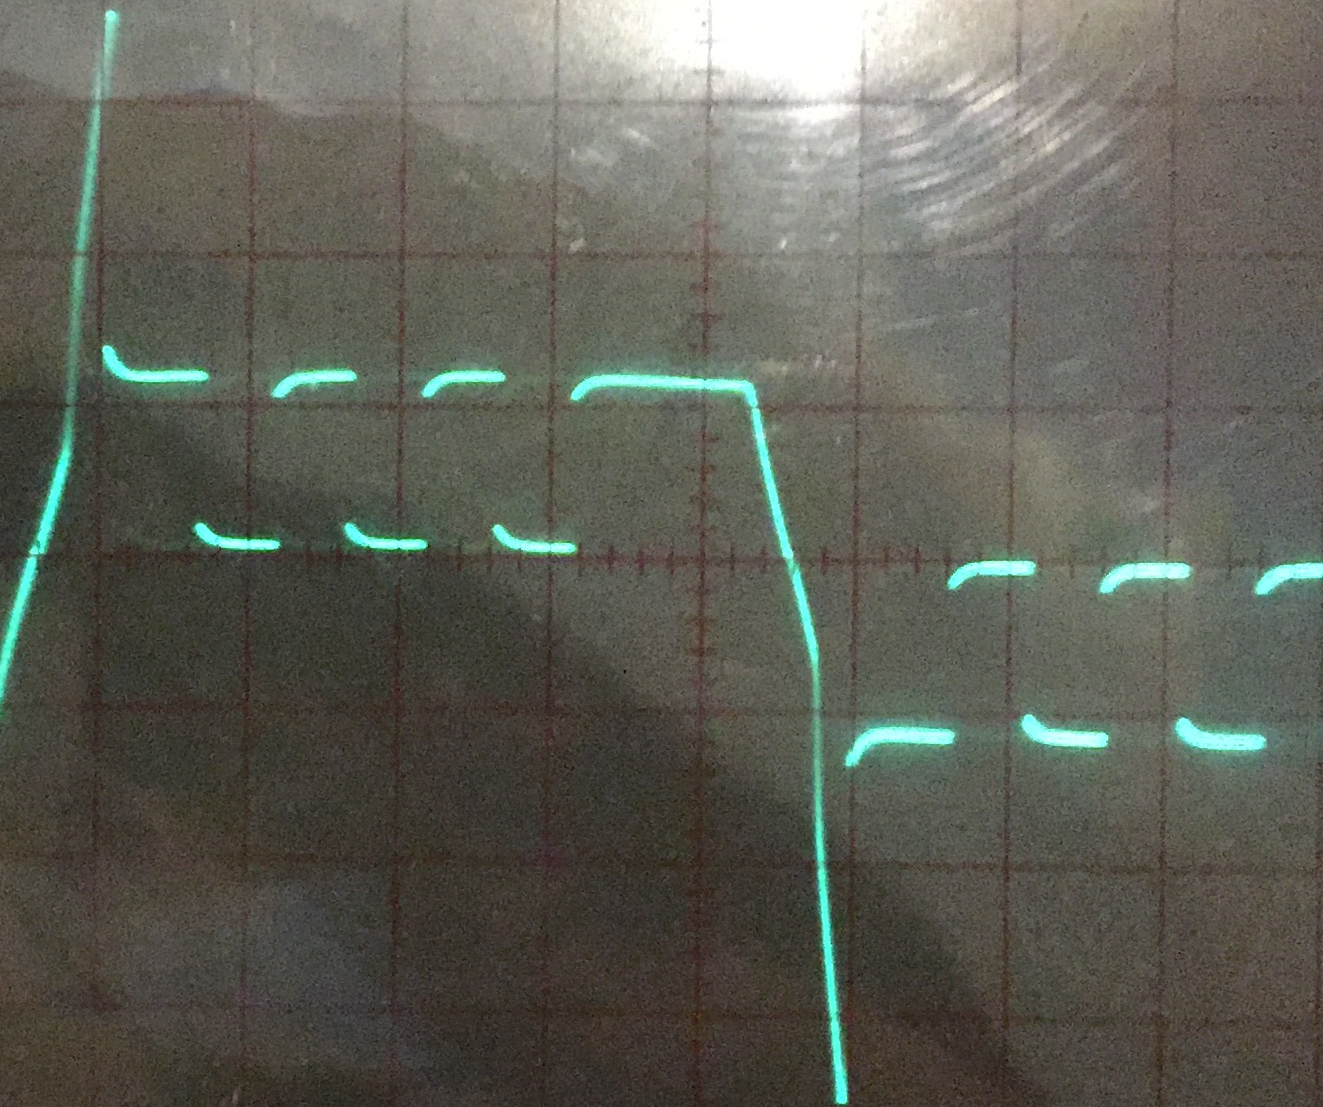
\includegraphics[width=0.6\textwidth]{../chapters/hardware-chapters/AC/ac-modulator/custom-hardware/ac-current-source/current-source-measurement-cropped.png}
		\end{figure}


	\end{frame}




	%\begin{frame}\frametitle{DC vs AC Voltage}
	%	\begin{figure}
	%		\resizebox {\textwidth} {!} {
	%		  \centering
	%		  \begin{minipage}[b]{0.49\textwidth}
	%		    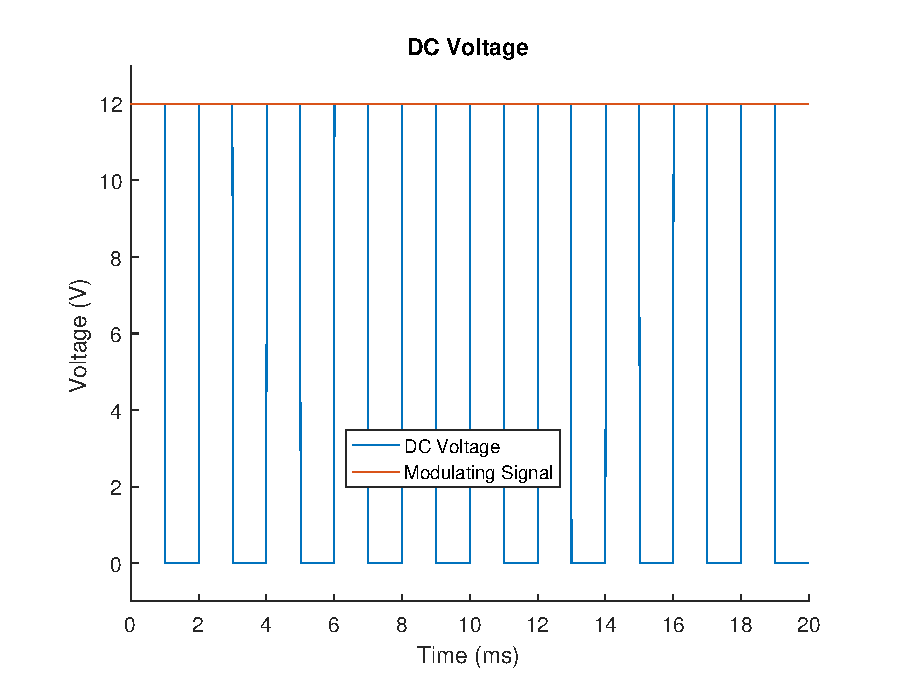
\includegraphics[width=\textwidth]{dc-wave.eps}
	%		  \end{minipage}
	%		  \hfill
	%		  \begin{minipage}[b]{0.49\textwidth}
	%		    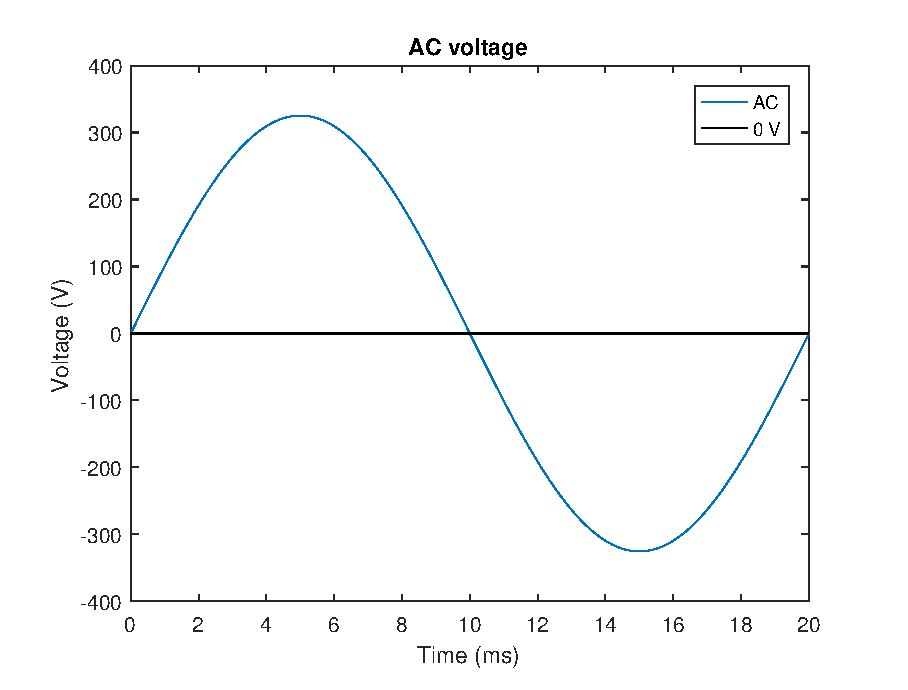
\includegraphics[width=\textwidth]{ac-wave.eps}
	%		  \end{minipage}
	%	  }
	%	\end{figure}
	%	AC characteristics:
	%	\begin{itemize}
	%		\item Supplied voltage is not constant.
	%		\item Supplied voltage will be both positive and negative.
	%	\end{itemize}
	%\end{frame}
	

	% Now that we are able to translate the ID into the nergy signature with this custom modulator,
	% we must also have a method of sampling the energy consumption.

	% this smart meter also consists of two important parts.
	% The part where it samples the current and gives this information to the microcontroller.
	% And also the same  triggering circuit is presetn to notify the micro controller when to start and stop looking for encoded information.


	\begin{frame}\frametitle{Smart-meter}
		
		\begin{figure}
			\centering
			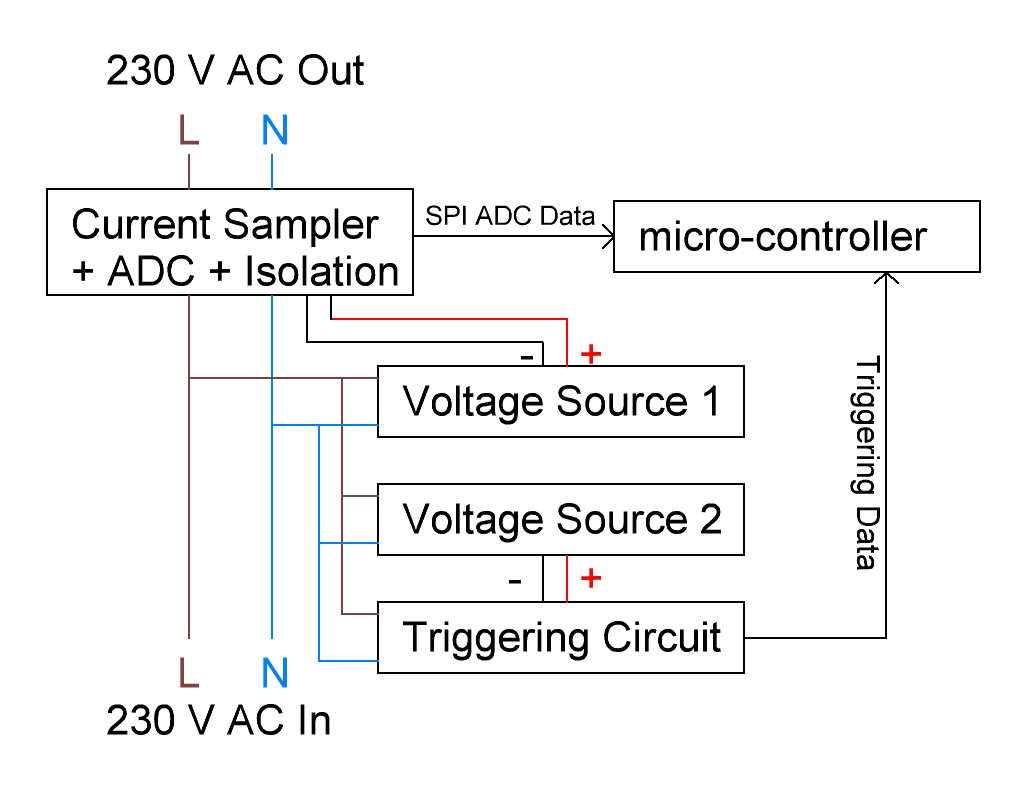
\includegraphics[width=0.8\textwidth]{../chapters/hardware-chapters/AC/ac-current-sampler/ac-current-sampler-architectural.JPG}
		\end{figure}

	\end{frame}
	



	%\begin{frame}\frametitle{Smart meter}
	%	AC Current sampler options:
	%	\begin{columns}
	%		\begin{column}{0.48\textwidth}
	%			\begin{itemize}
	%				\item Hall effect sensor:
	%				\begin{itemize}
	%					\item Sensitivity: 185 mV / A
	%					\item Noise: 21 mV
	%					\item Output: 15 W LED yields 12 mV 
	%					\item Noise $>$ output: not a viable option.
	%				\end{itemize}
	%				\item Burden resistor:
	%				\begin{itemize}
	%					\item Sensitivity: 2800 mV / A
	%					\item No noise 
	%					\item Output: 15 W LED yields 183 mV 
	%					\item Positive and negative voltage output %because of AC, so add a constant voltage to it and feed to an ADC
	%				\end{itemize}
	%			\end{itemize}
	%		\end{column}
	%		\begin{column}{0.48\textwidth}
	%			\begin{figure}
	%				\centering
	%				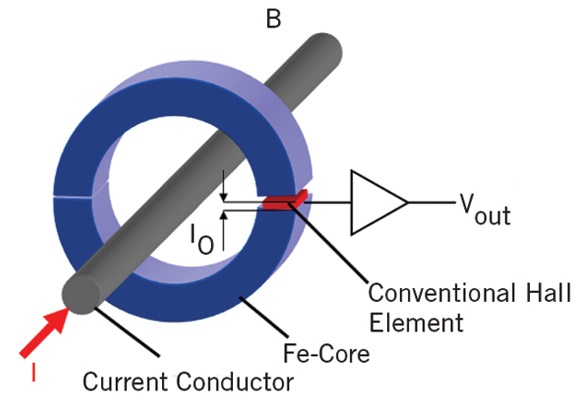
\includegraphics[width=0.8\textwidth]{hall-effect-sensing}
	%			\end{figure}
	%		\end{column}
	%	\end{columns}
	%\end{frame}



	% up to this point we have investigated the codes that we will use
	% And also the hardware to encode and decode the current has been explained
	% So now it is time to evaluate the etire system with all its components.


	\begin{frame}\frametitle{Recap}

		\begin{figure}
			\centering
			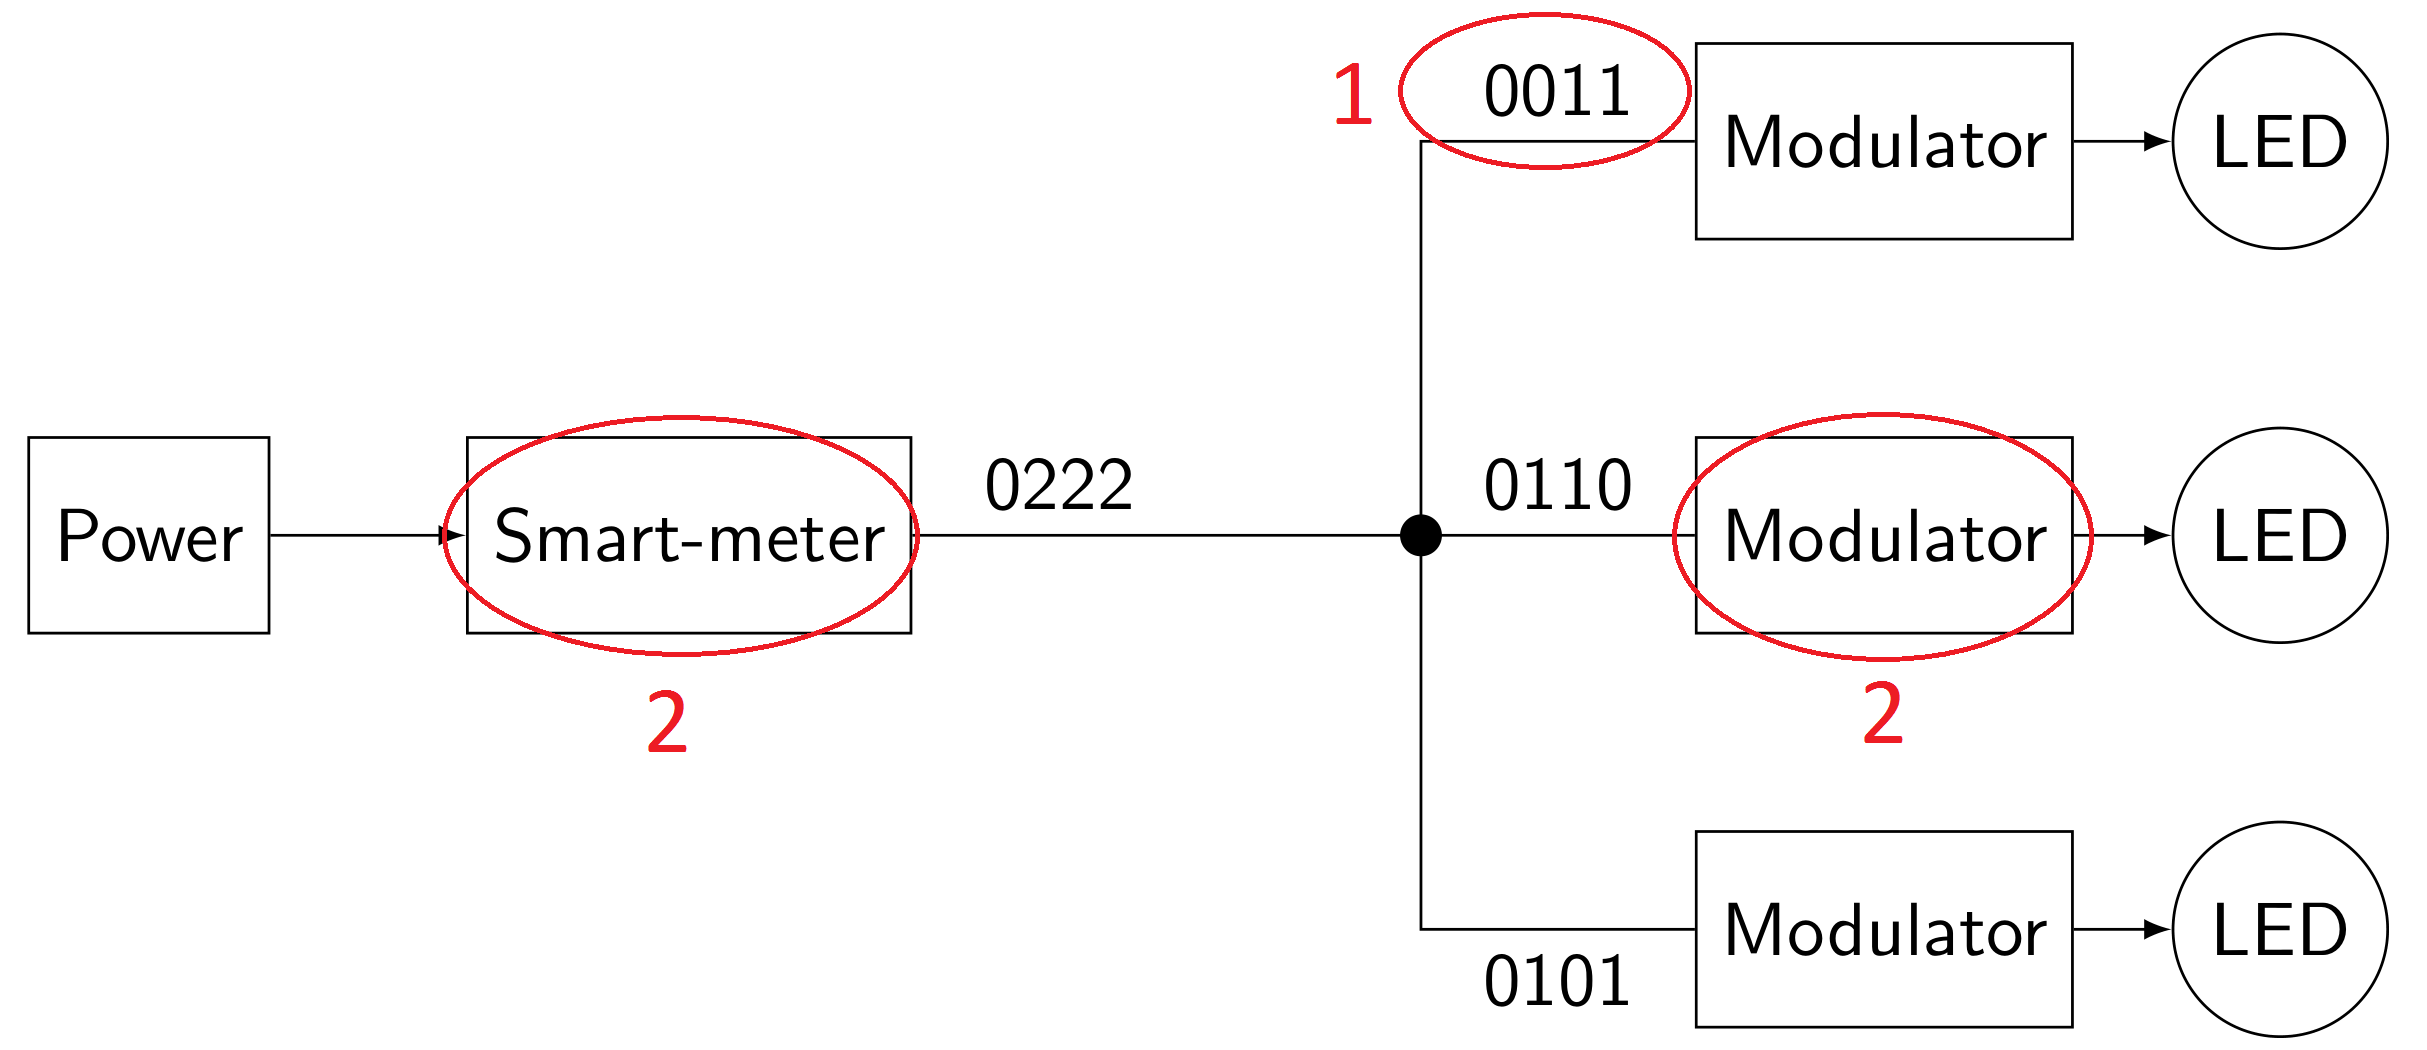
\includegraphics[width=\textwidth]{contributions-figure.png}
		\end{figure}
		\begin{enumerate}
				\item Codes
				\item Hardware
				\item Evaluate the system
		\end{enumerate}
		

	\end{frame}



	% We will perform a small scale evaluation with actual hardware and commercial LEDs.
	% To show the scalability of the system a software simultion will be performed.

	\begin{frame}\frametitle{Evaluation Outline}

		\begin{itemize}

			\item Hardware evaluation
			%\begin{itemize}
			%	\item Describe the setup.
			%	\item Explain the results.
			%\end{itemize}

			\item Software simulation
			%\begin{itemize}
			%	\item Describe the simulation.
			%	\item Discuss the results.
			%\end{itemize}

		\end{itemize}
	\end{frame}





	% this is what the ac testbed looks like with three commercial leds.
	% each led has its own modulator
	% and top left is the smart-meter.

	\begin{frame}\frametitle{AC Testbed}
		
		\begin{figure}
			\centering
			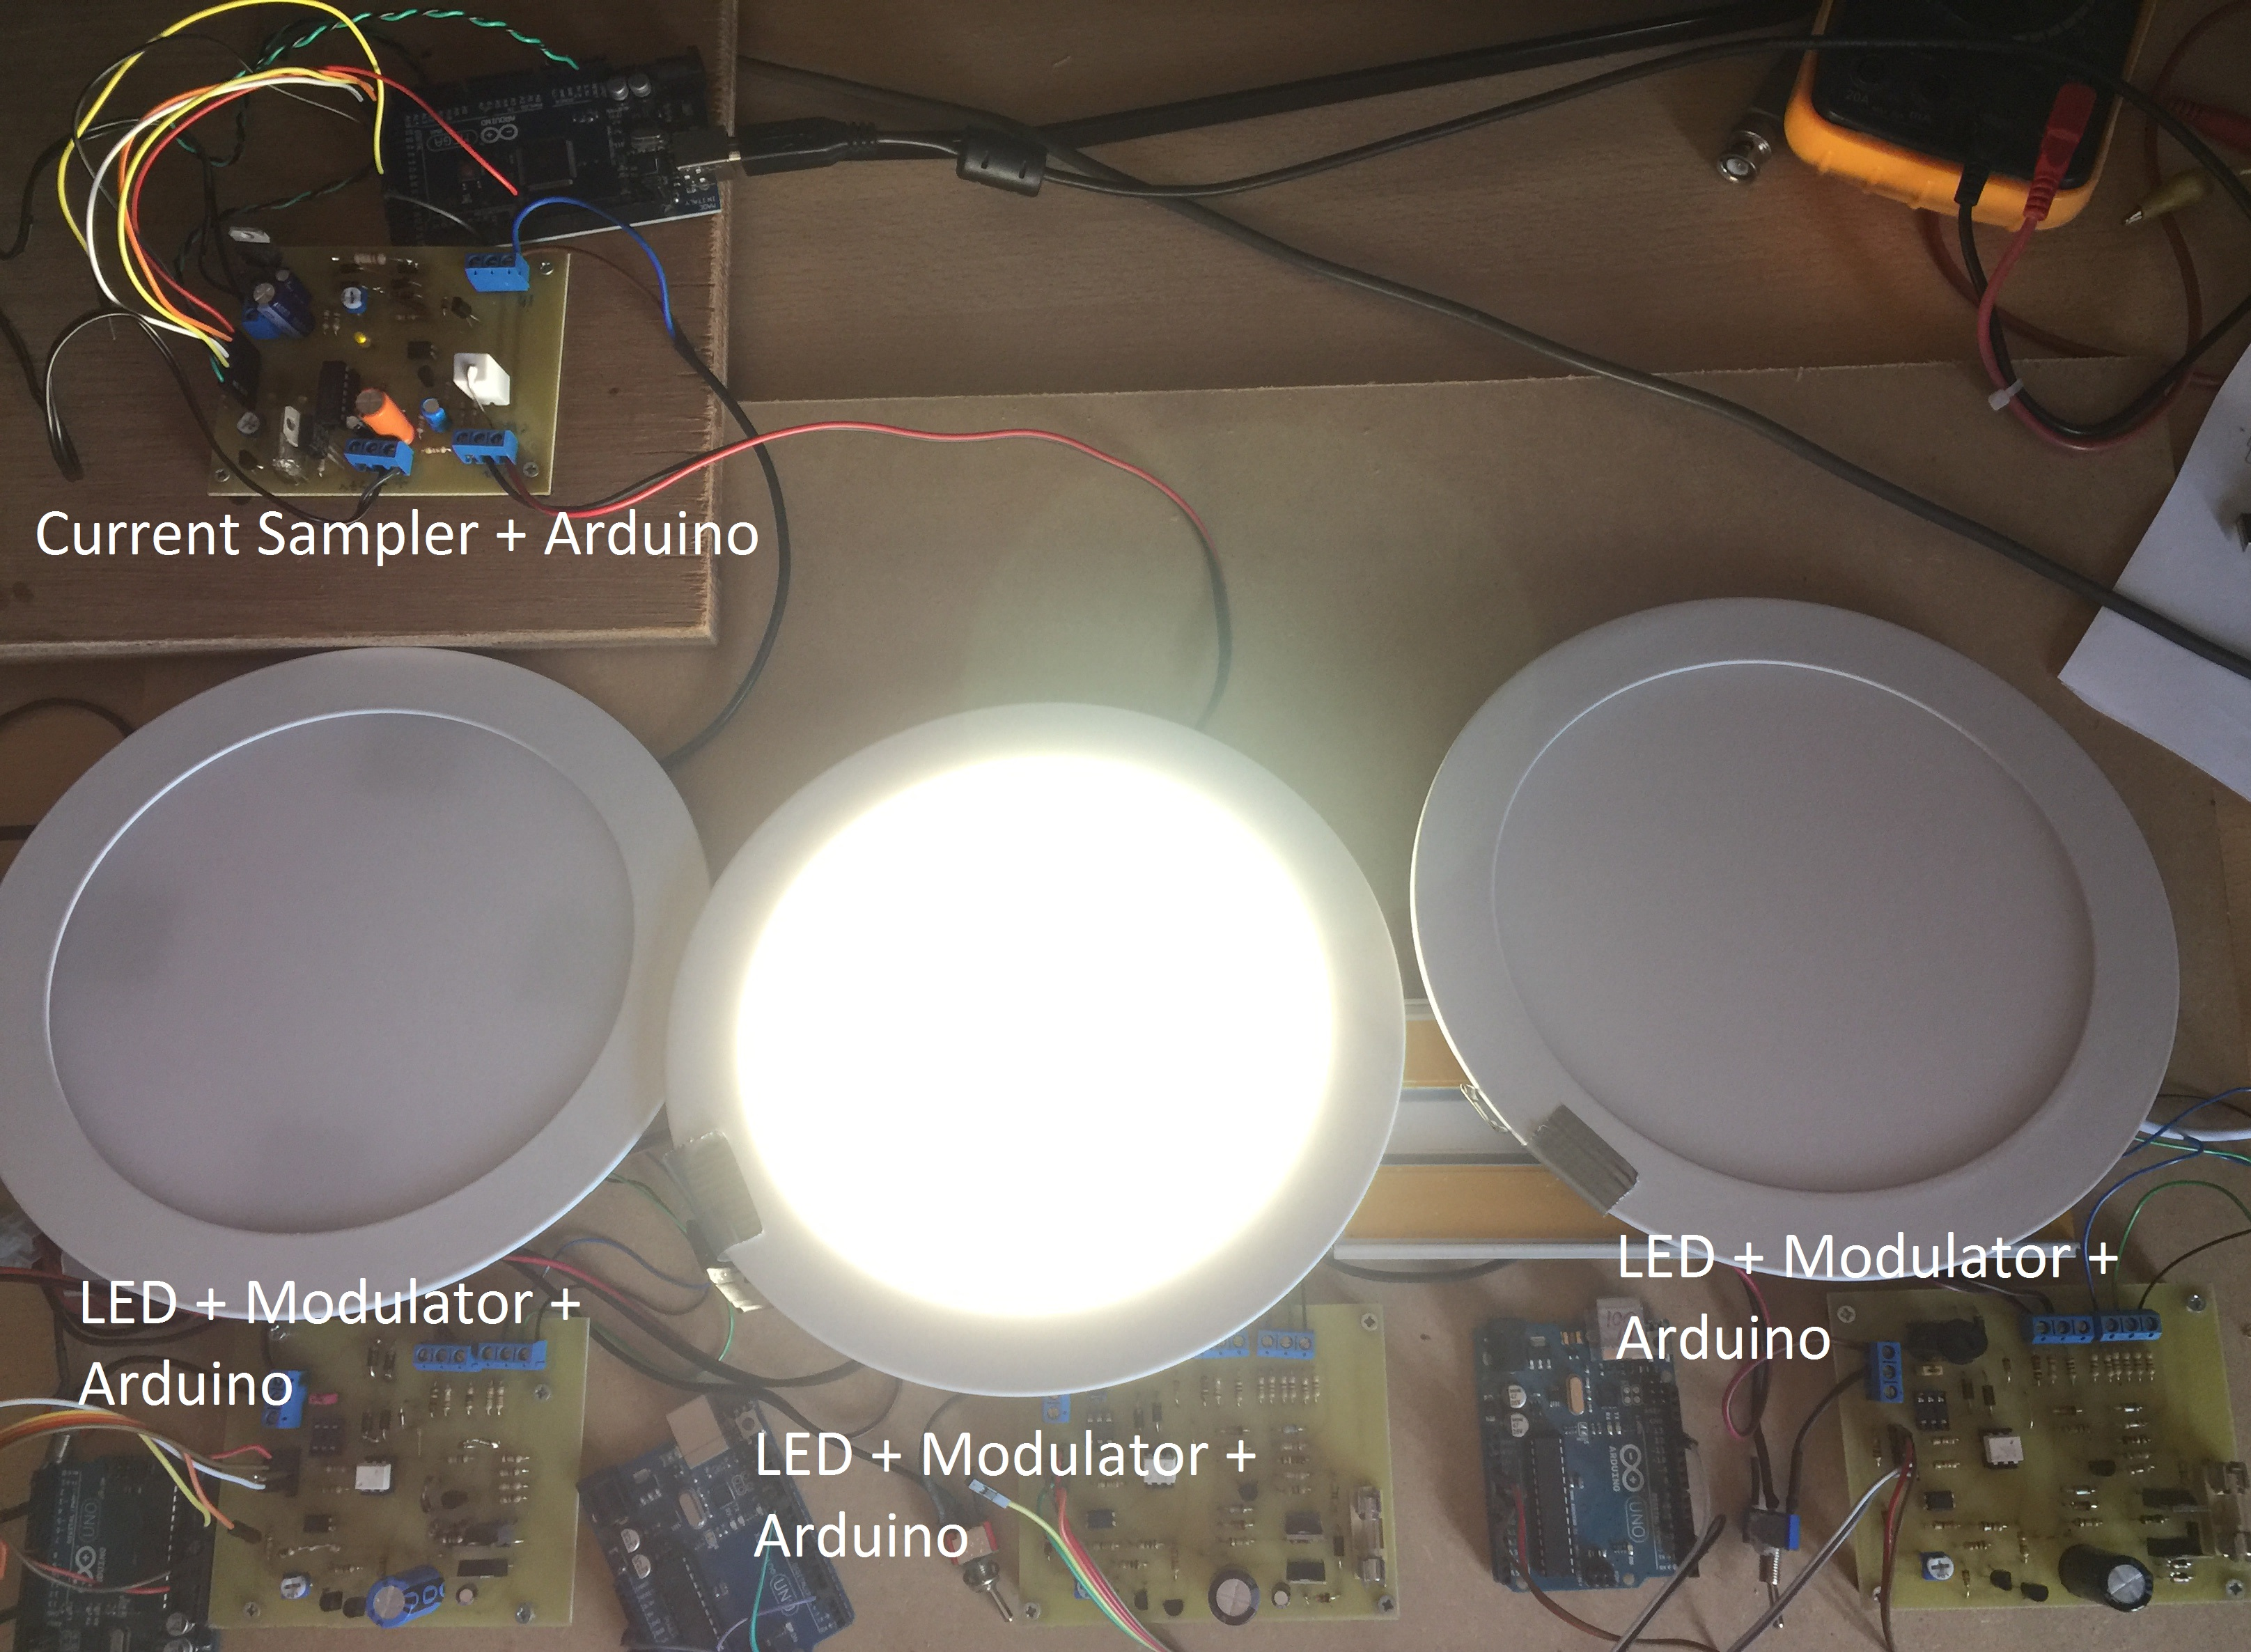
\includegraphics[width=0.8\textwidth]{../chapters/hardware-chapters/AC/ac-test-bed/ac-test-bed-picture}
		\end{figure}

	\end{frame}





	\begin{frame}\frametitle{Setup for Hardware Evaluation}
		
	
		\begin{itemize}

			\item Setup: 
			\begin{itemize}
				\item The setup consists of 3 commercial LEDs + current sampler.

				\item 4 distinct codes will be used, 3 for the LEDs and one will represent an LED in an off state.

				\item All LEDs are transmitting continuously with a code that support at least $m \ge 3$ concurrent transmitters.
			\end{itemize}

			\item Goals:
			\begin{itemize}
				\item Identifying an LED as being on without seeing interference from the other LEDs in a timely manner.

				\item Verify that the fourth code cannot be identified as being on. 

			\end{itemize}



		\end{itemize}
	\end{frame}



	% raw energy consumptio data can be seen here along with the triggering circuit output.
	% we can use the trigger to filter out the modulated data and process it.

	\begin{frame}\frametitle{Raw Data}

		\begin{figure}
			\centering
			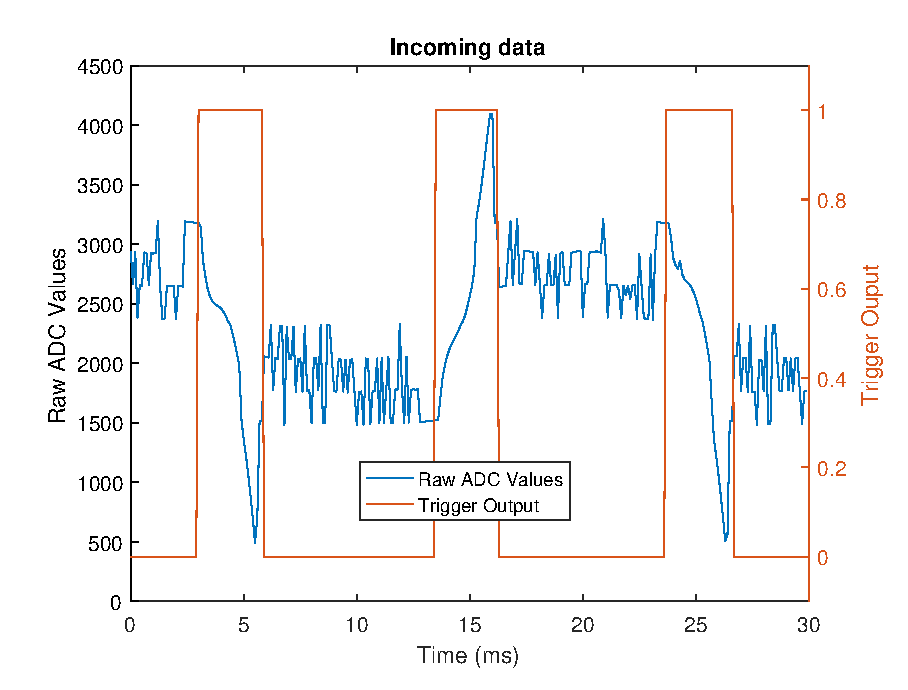
\includegraphics[width=0.8\textwidth]{ac-raw-data.eps}
		\end{figure}

	\end{frame}



	%When it is process it looks like this
	% where also the current flow is shown in the right y-axis 
	% from this figure we can see 4 distinct entries.
	% when all leds are mod. a 0 the current is approx. 0
	% when only 1 led is modualting a 1 the current is approx. 100 ma

	% and so on
	% We can use this data to find out if the leds are on or off by correlating the ID of the LED with this data.

	\begin{frame}\frametitle{Processed Data}

		\begin{figure}
			\centering
			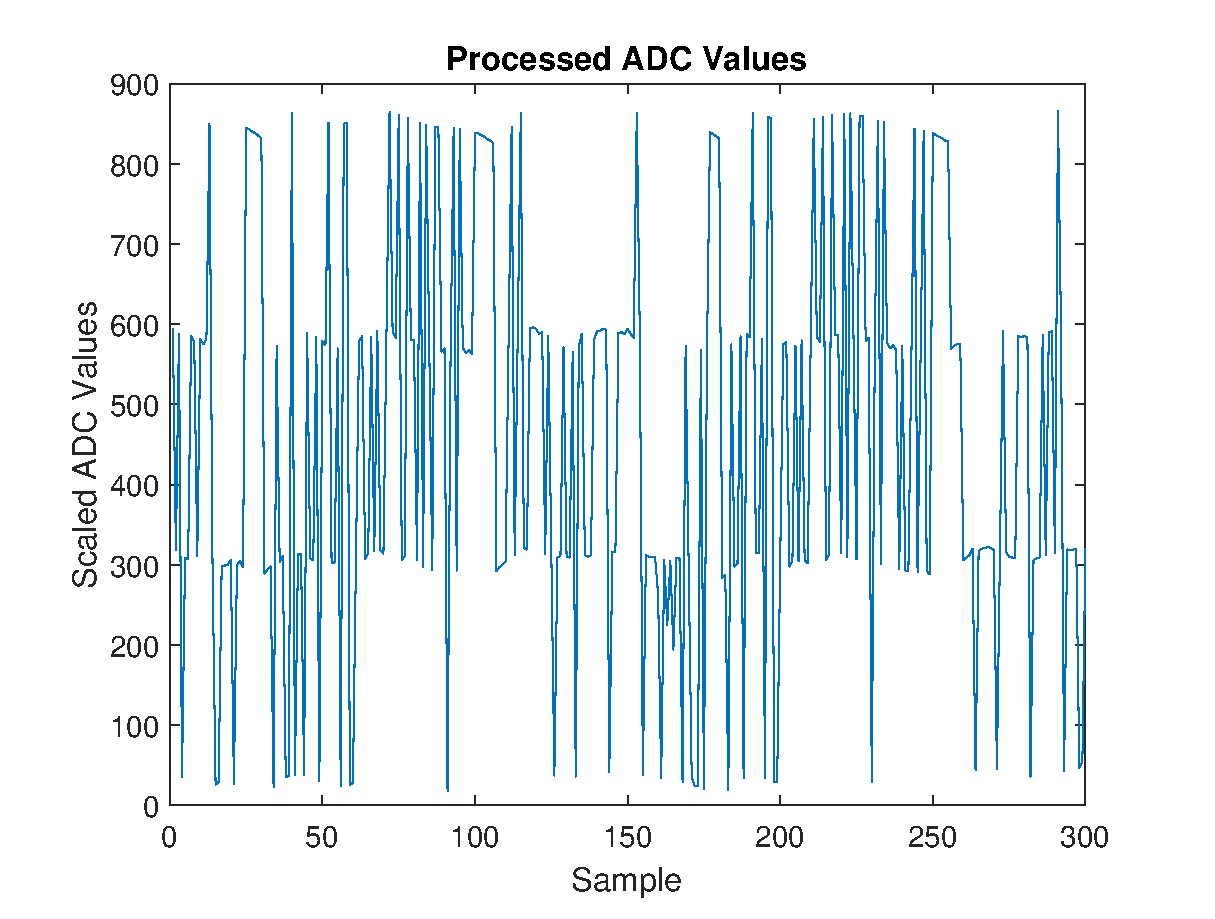
\includegraphics[width=0.8\textwidth]{../chapters/evaluation-chapters/hardware/ac/processed-ac-testbed-adc-data.eps}
		\end{figure}

	\end{frame}



	% First of we can see here the threshold line, if a results is above measn led on else led is off.

	% the blue signal represents the LED which is on and the oragne signal the led that is off.
	% from the blue signal we can see that the led is being identified as being on two times in less than 20 ms.
	% and the other led is identifeid as being offf, since it is below the threshols at all times.


	% now this was only a small scale system but the results are correct
	% to show the scalability a software simultion is performed.

	\begin{frame}\frametitle{Identifying LEDs}

		\begin{figure}
			\centering
			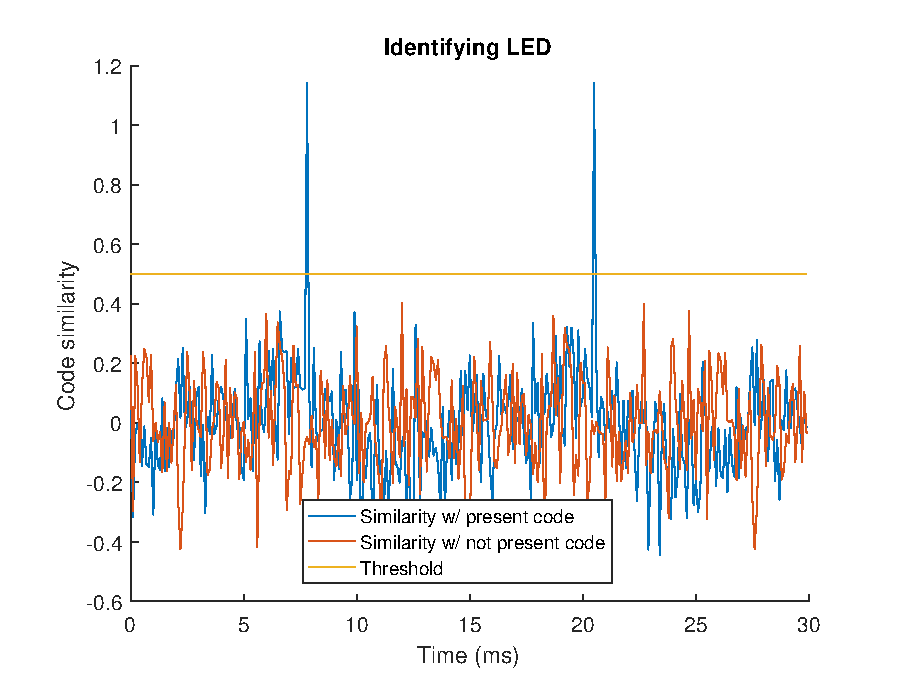
\includegraphics[width=0.8\textwidth]{correlation-results.eps}
		\end{figure}

	\end{frame}











	\begin{frame}\frametitle{Simulation}
		
		To be able to test larger systems, a software simulation is used: 

		\begin{itemize}

			\item Assuming 129 individual LEDs which follow the probabilistic scheme.

			\item Each LED has its probability $p$ for which it will modulate.

			\item Those LEDs will then transmit its code.

			\item The aggregated signal with all the code is then checked to try to identify if any LEDs are on.
		\end{itemize}

		

	\end{frame}




	%First a fast simulation is shown
	% This simulation is fast beacuse the accuracy is relatively low

	% As seen from this orange line all 129 leds have transmitted their IDs in less than a second.

	% the green dashed line represents m, the max. no. of modulating LEDs such that no interference issues occur.
	% whenever the no., of .modulating leds represneted by the blue dots is below the green line, we can guarntuiee the accuracy of the system
	% As seen from this first part when the blue dots stay below the green line, the accuracy represented by the red line is 100 %.

	% When the no. of modualting leds is more than it may or may not happen that we get errors.
	% as seen from the last part of the figure. the blue dots are above the green line and yet thre accuacy is till 100 %

	% we can see the errors in the moiddel part of the figure.
	% here the blue dots are also above the m line and the accuracy drops.
	% The accuracy can drop bacause leds are mistakenly idetified as being on when they are acyally off and vice versa.

	% so this was a fast sim but relatively in accuarte

	\begin{frame}\frametitle{Fast but Inaccurate Simulation}
		
		\begin{figure}
			\centering
			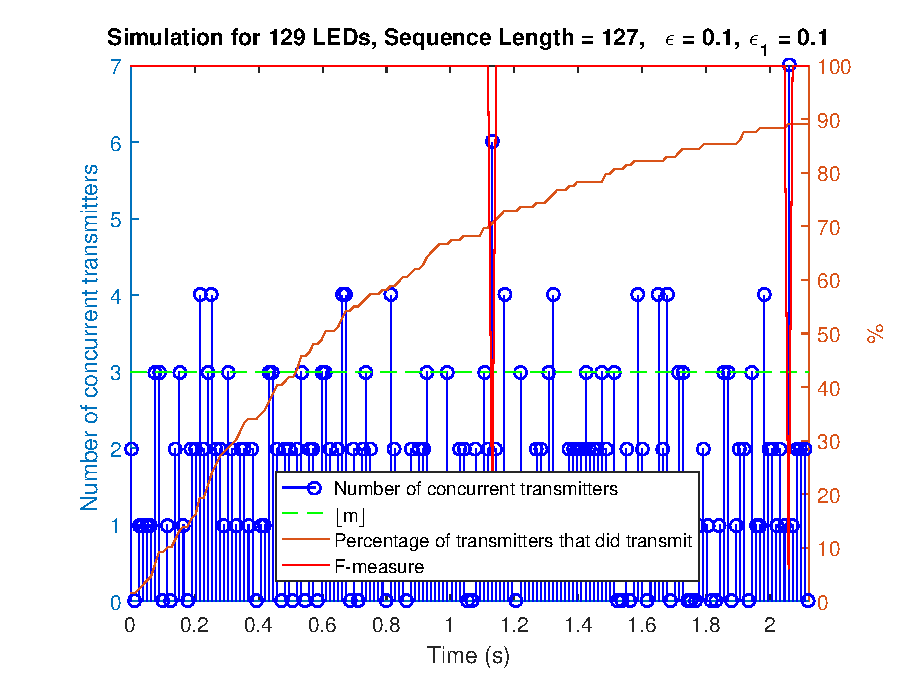
\includegraphics[width=0.8\textwidth]{../chapters/evaluation-chapters/simulation/sim-concurrent-tx-and-f-measure-eps=1-n=7}
		\end{figure}

	\end{frame}


	% here a slower simulation but more accurate.
	% here we can see from the orange line it takes all the 129 leds roughly 4 seconds to transmite their IDs.
	% so this is 4 times slower.
	% but the no. of modualting leds always is on or below the green line, so the accuracy is 100 % 

	% so this is a slower but more accurate sim and proves the scalability of the system

	% and with that being said we ve reached the conclusion,.

	\begin{frame}\frametitle{Slow but Accurate Simulation}
		
		\begin{figure}
			\centering
			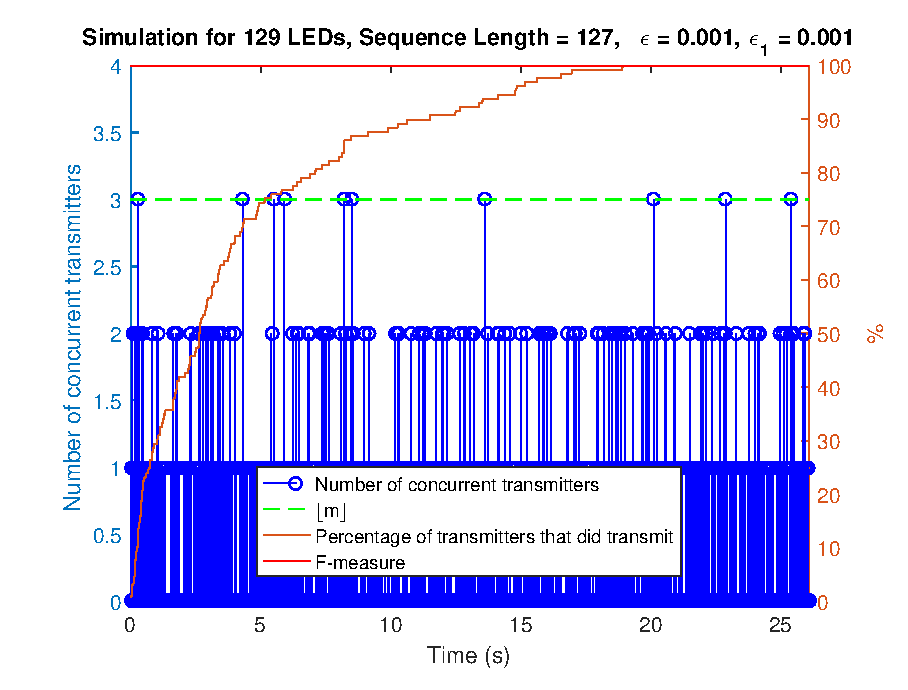
\includegraphics[width=0.8\textwidth]{../chapters/evaluation-chapters/simulation/sim-concurrent-tx-and-f-measure-eps=001-n=7}
		\end{figure}

	\end{frame}




	% Investigatd codes and made them suitable for the use with LEDs.
	% Designed hardware to give each LED a recognizable and unique energy signature.
	% Designed smart-meter which can sample the aggregated energy consumption.
	% Made software which can detect which leds are on by looking at the aggragted energy consumption
	% PRoven the scalability of the system.

	% two most important items for future work are to do with other appliances and dimming lights.

	% When other appliances are also used we must evaulate if the leds can still be relabley detected.
	% giving the fact that lights modualte at specfic frequency we could filter out this frequency adn see if the leds can be reliably detected.S

	% LEds are often too bright for a poerson liking.
	% so these leds must be dimmed
	% however by dimming these lights the amplitude of the current chages and the codes are designed to work when all codes have the same apmplitude.
	% possible solution is to use a different mod. freq. for each dimming level and filter the maccordingly .


	\begin{frame}\frametitle{Conclusion and Future Work}

		\begin{itemize}
			\item Conclusion:
				\begin{itemize}

					\item Codes have been investigated.

					\item Hardware is designed to encode and decode the IDs.

					\item The software and hardware is evaluated along with a simulation for scalability.

				\end{itemize}

			\item Future Work:
				\begin{itemize}

					\item Other appliances

					\item Dimming lights

				\end{itemize}
		\end{itemize}

		
		
		

	\end{frame}












\end{document}
